\documentclass[a4paper,11pt]{article}

% \usepackage{showkeys}
\usepackage[english]{babel}
\usepackage[style=apa6]{biblatex}
\usepackage[utf8]{inputenc}
\usepackage[document]{ragged2e}
\usepackage{setspace}
\usepackage{geometry}
\usepackage{mathptmx}
\usepackage{rotating, graphicx}
\usepackage{float}
\usepackage{multicol}
\usepackage[hidelinks]{hyperref}
\usepackage[scaled]{helvet}
\usepackage[T1]{fontenc}
\usepackage{fancyhdr}
\usepackage[labelsep=period]{caption}
\usepackage{titlesec}
\usepackage{tocloft}
\usepackage{titletoc}

\fontfamily{phv}\selectfont

\newcommand{\thesistitle}{
	CodeNect: Visual Programming Software for\\
	Learning Fundamentals of\\
	Programming}

\newcommand{\thesisautors}{
	\textbf{Lim-it, Brandon B.,}\\
	\textbf{Punay, Jaykel O.}\\}

\captionsetup{justification=centering}
\renewcommand{\cftsecleader}{\cftdotfill{\cftdotsep}}

\fancypagestyle{plain}{
	\fancyhf{}
	\renewcommand{\headrulewidth}{0pt}
	\renewcommand{\footrulewidth}{0pt}
}

\renewcommand*\familydefault{\sfdefault}
\addbibresource{bibliography.bib}

\singlespacing
\pagestyle{myheadings}
 \geometry{
	a4paper,
	lmargin=1.5in,
	rmargin=1in,
	tmargin=1in,
	bmargin=1in,
}

\newcommand{\parx}{
	\setlength{\parindent}{4em}
	\par}

\newcommand{\listappfigname}{
	\normalsize\textbf{LIST OF APPENDIX FIGURES}\par
	\flushleft\textbf{Appendix}\\
	\textbf{Figure}\hfill\textbf{Page}
}
\newlistof{appfig}{appf}{\listappfigname}
\newcommand{\appfig}[1]{
	\refstepcounter{appfig}
	\par\noindent\normalsize{\theappfig. #1}
	\addcontentsline{appf}{appfig}
	% {\protect#1}\par
	% {\protect\numberline{\thesection.\theappfig} #1}\par
	{\protect\numberline{\theappfig} #1}\par
}

\newcommand{\appendixdata}[1]{
	\begin{figure}[H]
		\centering
		\includegraphics[width=0.8\textwidth]{figures/results/#1.png}
		% \caption{dataresults#1}
		% \label{fig:dataresults#1}
	\end{figure}
}

\newcommand{\appendixform}[2]{
	\begin{figure}[H]
		\centering
		\includegraphics[width=\textwidth]{figures/form#1/form#2.jpg}
		\label{fig:form#2}
	\end{figure}
}

\newcommand{\listappname}{
	\normalsize\textbf{LIST OF APPENDICES}\par
	\textbf{Appendix}\hfill\textbf{Page}
}
\newlistof{app}{appp}{\listappname}
\newcommand{\app}[1]{
	\refstepcounter{app}
	\par\noindent\normalsize{Appendix \theapp. #1}
	\addcontentsline{appp}{app}
	% {\protect#1}\par
	{\protect\numberline{\theapp} #1}\par
}

\titleformat{\section}{\center{\normalfont\normalsize\bfseries}}{}{0pt}{}
\titleformat{\subsection}{\center{\normalfont\normalsize\bfseries}}{}{0pt}{}

\newcommand{\fakesection}[1]{
	\par\refstepcounter{section}
	\sectionmark{#1}
	\addcontentsline{toc}{section}{\protect\numberline{\thesection}#1}
}

\newcommand{\fakesubsection}[1]{
	\par\refstepcounter{subsection}
	\subsectionmark{#1}
	\addcontentsline{toc}{subsection}{\protect\numberline{\thesubsection}#1}
}

\begin{document}
	\addtocontents{toc}{~\hfill\textbf{Page}\par}

\begin{singlespace}
	\begin{titlepage}
		\begin{center}
			\textbf{\thesistitle{}}

			\vfill
			\center
			An Undergraduate Thesis\\
			Submitted to the Faculty of the\\
			College of Engineering and Information Technology\\
			Cavite State University\\
			Indang, Cavite

			\vfill
			\center
			In partial fulfilment\\
			of the requirements for the degree\\
			Bachelor of Science in Information Technology

			\vfill
			\thesisautors{}
			{June 2021}

		\end{center}
	\end{titlepage}
\end{singlespace}


	\clearpage
	\renewcommand{\contentsname}{\hfill\normalfont\normalsize \textbf{TABLE OF CONTENTS}\hfill}
	\renewcommand{\cftaftertoctitle}{\hfill}

	\pagenumbering{roman}
	\setlength{\cftbeforesecskip}{12pt}
	\setlength{\cftbeforesubsecskip}{12pt}
	\renewcommand{\thesection}{}
	\renewcommand{\thesubsection}{}
	\tableofcontents

	\clearpage
	\fakesection{\textbf{LIST OF FIGURES}}
	\renewcommand{\listfigurename}{\hfill\normalfont\normalsize \textbf{LIST OF FIGURES}\hfill}
	\addtocontents{lof}{~\textbf{Figure}\hfill\textbf{Page}\par}
	\pagenumbering{arabic}
	\doublespacing
	\listoffigures
	\singlespacing

	\clearpage
	\fakesection{\textbf{LIST OF APPENDIX FIGURES}}
	\pagenumbering{arabic}
	\begin{center}
		\doublespacing
		\listofappfig
		\singlespacing
	\end{center}

	\clearpage
	\fakesection{\textbf{LIST OF APPENDICES}}
	\pagenumbering{arabic}
	\begin{center}
		\doublespacing
		\listofapp
		\singlespacing
	\end{center}

	\clearpage
	\pagenumbering{arabic}
	\begin{center}
	\textbf{\thesistitle{}}

	\leavevmode\\
	\leavevmode\\

	\thesisautors{}

	\leavevmode\\
	\leavevmode\\

	\hrule
	\parbox{\textwidth}{
	\justify
	An undergraduate thesis outline submitted to the faculty of the Department of Information
	Technology, College of Engineering and Information Technology, Cavite State University,
	Indang, Cavite, in partial fulfillment of the requirements for the degree of Bachelor of
	Science in Information Technology. Pre-pared under the supervision of Mr. James Angelo V. Aves}
	\hrule

	\leavevmode\\
	\leavevmode\\
\end{center}


\begin{doublespace}
	\thispagestyle{empty}
	\begin{center}
		\section{\textbf{INTRODUCTION}}
	\end{center}

	\fakesubsection{Background of the Study}
	\justifying
\parx
As the innovation in technology is continuously making its progress in improving
the quality of life. With this nature of technology comes the essential need for
programming skill as core profiency. The competition in the field that
developers and programmers alike strive for is becoming harder to get into due
to high standards and requirements. One of the requirements for a programmer and
developer is to have expertise in technical skills that include multiple
programming languages (\cite{tsai_yang_chang_2015}). Without the proper
knowledge and understanding in programming in its fundamental level and depth,
one will find it difficult to adapt to the constantly shifting world of
computer.

\parx
Improving learning without prolonging the time allotted in each
academic year needs to focus on enhancing the properties of the software that
are both utilized as teaching and learning tools by the instructor and the
student. A system that is implemented using modern tools, industry
standard design, and functionality that focuses in simplicity, readability, and
learning experience. Modern technology increases the rate of knowledge
acquisition and absorption through its usage and implementation in education
(\cite{raja_nagasubramani_2018}). The advancement in technology greatly
contributes to education as it enables convenience in communication and
presentation of knowledge and information almost instantaneously
(\cite{anggrawan_ibrahim_m}). A software that prioritize functionality over
unnecessary features to ensure that the user is not overloaded with information
in the screen that is unnecessary. Users perceive numerous features in a product
to be useful and engaging but such can result in fatigue
(\cite{thompson_hamilton_rust_2005}).

\parx
Software with the necessary tools and functionalities oriented towards learning
purposes and is also designed to and packaged with coding exercises and problems
which range from beginner, intermediate, to advance difficulties is not popular
and lacking in availability. Features that are carefully selected and designed
towards showing and comparing various solutions that are working in the context
that they meet the requirements and output and are technically correct, but not
all will meet the standard when it comes to better quality which is the
advantages in skills acquired when mastering the fundamentals of programming.
This approach in problem solving allows learners to develop logical and critical
thinking through the application of the theory of variation, wherein some
aspects that are critical must vary while other aspects stay constant
(\cite{cheng_2016}). This is effective in the domain of programming as even a
slight change in data amounts to a change in effect and output.

\parx
Programming is a skill wherein it focuses in the connection of logic rather than
memorizing information as that of in other domain, the curve in starting to
learn it is steeper compared to actually applying it in real works and mastering
it. Mastering a programming language is not an easy task, but in general all
share common concepts. Learning by heart these core concepts and fundamental
knowledge will help programmers to easily learn and master any existing or new
programming language through the reiteration of principles that all programming
languages are built and modeled upon. For the design and decision that go behind
the creation of new programming languages are reevaluation of existing studies,
syntax, semantics, and inspired by widely used and accepted languages
(\cite{stefik_siebert_slattery_stefik_2011}). For anyone who is new to
programming, the topics can be a daunting and intimidating task. Failure in
familiarization and application in the early academic years and progressing to
the next period wherein advance subjects are covered bereaves the overall
learning of the student.

% \parx
% The integration of a visual nodes and graphs as the interface in programming instead
% of the traditional text-based language is simpler, more appealing to use, and more
% intuitive to get started with. Visual programming saves time in specifying the code
% textually and manually input. It enables learning through interaction and manipulation
% of graphical elements which can provide more feedback through the use of color, size,
% and icons. The abstract and high-level concepts are represented visually that can
% facilitate learners by variable observation, logic flow tracing, and debugging skills
% (\cite{tsai_yang_chang_2015}). This visual programming tool can also export an
% equivalent source code to other programming languages that are in the curriculum
% such as C/C++, Java, and Python. The tandem of visual code and textual code allows
% programmers to write programs while learning fundamental concepts as seeing the code
% in both formats. This allows to ease the transition from introductory visual programming
% skill to real text-based programming language. (\cite{alam_bush_2016})


	\fakesubsection{Statement of the Problem}
	\flushleft
\textbf{Statement of the Problem}\\

\justifying
\parx
The fundamental concepts of programming are essential basics that are necessary
for programmers to master. Concepts such as syntax, semantics, variables, data
types, data structures, logic, conditionals, loops, algorithm, and memory are
key to easily understanding and getting better at programming as it is a
discipline (\cite{prahofer_hurnaus_wirth_mossenbock_2007}).
Programming is a skill which can be boring, intimidating, and unrelated to daily
activities and experience. Students are lacking in understanding of the
execution of a program (\cite{tan_2019}).
Programming education requires the assistance of technology itself through
software in improving the quality of learning. The traditional method of pure
lecture is nowadays complimented with the application of software. But most
tools are not beginner-friendly and are cluttered with features that present
confusion and steep learning curve in familiarity and mastery that diminish the
learning experience (\cite{tsukamoto_2016}).

\justifying
\parx
The assessment of the respondents under the courses with programming subjects
(See Appendix Figure \ref{dataresults1}) shows that students (See Appendix
Figure \ref{dataresults13})
are not familiar and not well versed on fundamental concepts and find it
difficult to understand
(See Appendix Figure \ref{dataresults12} and \ref{fishbone1}).

\parx
Basic concepts such as loops, memory management, and functions are easily
understood individually, but combining them into a program has confused
students (See Appendix Figure \ref{fishbone2}). Respondents obtained low score
in the assessment questions (See Appendix Figure \ref{dataresults13}).

\parx
Survey shows that 76\% of students use text-based editors in their laboratory
classes such as Notepad++, DevC++, and TurboC/C++, while 24\% use professional
and modern editors (See Appendix Figure \ref{dataresults9}). These software are
general programming tools and are not oriented for assisting beginners in
learning fundamental concepts of programming (See Appendix Figure
\ref{fishbone3}).


	\fakesubsection{Objectives of the Study}
	\flushleft
\textbf{Objectives of the Study}\\
\justifying
\parx
The general objective of the study is to develop a CodeNect: Visual Programming
Software that will help in learning the fundamentals of programming.

\parx
Specifically, this study seeks:

\begin{enumerate}
	\item Identify the concepts learners find difficult to understand through conducted survey.
	\item Analyze the problems through data gathering.
	\item Design the system with the following features:
		\begin{enumerate}
			\item Visual Nodes Module handles the core elements and building blocks
				in the software for writing logic and code.
			\item Filesystem Module handles the creation, modification, reading, and
				deletion of files.
			\item Input and Output Module is the interface for user actions such as mouse
				events and key events and what is displayed to the screen for the user.
			\item Debug Module lints the visual code for errors and warnings before
				the running the code. It also captures errors and warnings during runtime
				and report it to the user.
			\item Simulation Module for compiling and running the visual program to
				a command line program.
			\item Transpiler Module that will convert the visual logic to other
				programming languages such as C/C++, Java, Python, Javascript, Lua, and
				more.
			\item Assessment Module that will evaluate the knowledge and learning of the
				users by providing basic and common coding exercises. Exercises can be
				imported, shared, and distributed through simple package files.
		\end{enumerate}

	\item Develop the system as designed.
	\item Test and improve the usability, functionality of the software using Experience-based test design.
	\item Evaluate the acceptability of the software using the ISO/IEC/IEEE 29119-4.2015. \\
\end{enumerate}


	\fakesubsection{Significance of the Study}
	\flushleft
\textbf{Significance of the Study}\\
\justifying
\parx
The result of the study will be of great benefits to the following:

\parx
The software will help in the education and improvement in the knowledge,
skills, understanding, and expertise of the students and learners about
programming. Thus, allowing them to compete and increasing the opportunities for
their careers.

\parx
The software will provide assistance for teachers and instructors to teach and
demo programming concepts through visualization. This will aid in relieving
workload, stress, and maximizing lessons each class time.

\parx
The software will benefit educational institutions like university for computer
laboratory classes by providing a free software oriented for the purpose of
learning.

\parx
The software will provide learning experience for the developers and researchers
in preparation for software development career.

\parx
This study would serve as a guide and reference in the field of software
development and education for future researchers.\\


	\fakesubsection{Conceptual Framework of the Study}
	\flushleft
\textbf{Conceptual Framework of the Study}\\

\justifying
\parx
The conceptual framework (refer to Figure \ref{fig:conceptual_framework}) represents the relationship
and flow of the concept of developing a visual programming software for learning the
fundamentals of programming.

\parx
It shows the order of actions required by the study to achieve the desired
output following the design of the context diagram (refer to Figure \ref{fig:context_diagram})

\parx
The inputs has the following requirements for the development of the study.
Knowledge requirements include programming, programming languages, parsing,
evaluation, C++ programming language, user-interface design, user-experience
design, data flow diagram, and context diagram.  Software requirement include
Linux 5.4 - Manjaro as operating system and distribution, Vim as text and code
editor, terminal, OpenGL and GLFW library for graphics and inputs, TinyC
Compiler for running the transpiled code at runtime, and the C++ programming
language for development. Microsoft Windows 7 and above, C++ Runtime libraries,
and the C++ programming language for deployment.  Hardware requirement are
machine with at at least Intel Core 2 Duo at 1.4 GHz, 2 GB of RAM, and 80 GB
HDD storage for development. At least Intel Core 2 Duo at 1.4 GHz, 2 GB of RAM,
and at least 1 GB HDD storage space for deployment.

\parx
The process to be followed and used for the development of the software is the V model.
The process model involves the requirements of gathering necessary data and information
from respondents through conducted survey. High-level design of the implementation of
the requirements of its technical usage for system design. Design of the relationships
and dependencies of the modules, creation of diagrams, and selection of technology to
be used. Preparation of the design and test method for each module. Followed by the
coding of the modules and the software. The evaluation is based on the ISO/IEC/IEEE
29119-4.2015, specifically the experience-based test design technique, to assure the
functionality, efficiency, usability, portability, and reliability of the software.

\parx
The impact expected from the study is the availability of a software designed for
learning to program and its fundamentals for learners, students, and educators.
Another impact is the improvements in the understanding, skills, and academic
performances of the students in the course of programming.

\begin{figure}[H]
	\centering
	\captionsetup{justification=centering}
	\captionsetup[figure]{list=yes}
	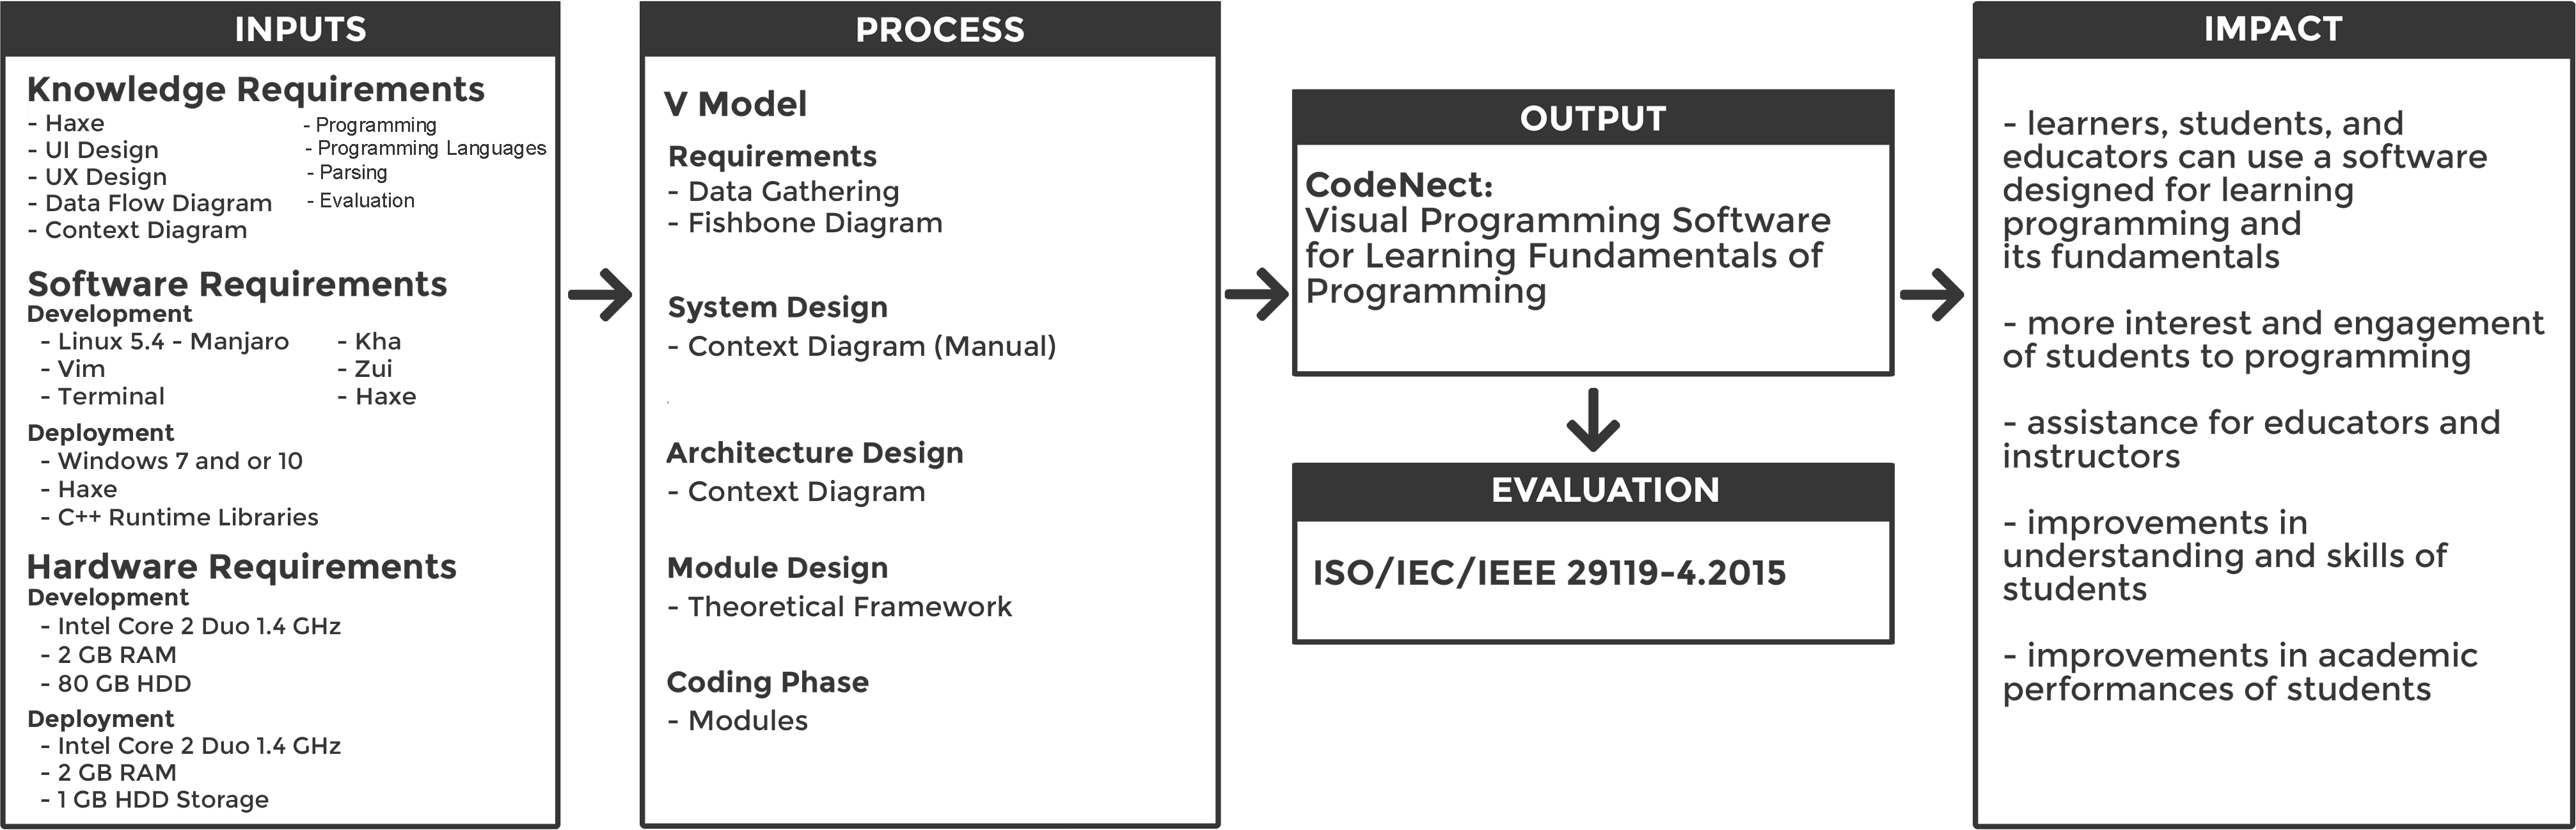
\includegraphics[width=\linewidth]{figures/conceptual_framework.png}
	\caption[Conceptual Framework]{Conceptual Framework of proposed CodeNect: Visual Programming Software for Learning Fundamentals of Programming}
	\label{fig:conceptual_framework}
\end{figure}


	\fakesubsection{Time and Place of the Study}
	\flushleft
\textbf{Time and Place of the Study}\\
\justifying
\parx
The study started from the approval of the title on the month of February of year
2020. The development is expected to be finished on the month of May of year
2021. The necessary data were gathered through survey and research at the Cavite
State University and other information were researched and obtained from the
Internet.\\


	\fakesubsection{Scope and Limitation}
	\flushleft
\textbf{Scope and Limitations of the Study}\\
\justifying
\parx
The study focuses on the development of a CodeNect: Visual Programming Software
for learning the fundamentals of programming. The software will prioritize
simple and basic functionalities over numerous features for the purpose of
learning and education.

The software is to be developed in Linux operating system using the C++ programming
language, Vim as code editor, terminal for building, Kha and the zui framework for
rendering.
The source is to be released as open-source with appropriate license to improve
contributions. Since the software is stand-alone desktop program, there will be no
account management. The software is only accessible by a single user such as the
student or instructor.
The software fully works in offline mode.

The software is designed with seven core modules: Visual Nodes Module,
Filesystem Module, Input and Output Module, Debug Module, Simulation Module,
Transpiler Module, and Assessment Module.

\flushleft
\textbf{\textit{Visual Nodes Module}}\\
\justifying
\parx
Nodes are graphical elements that serve as the building blocks of the software.
Nodes can be used as a variable, logic, and conditionals. The properties of the node
are position, size, and type. The fields of the node that are visible to the
users, which can be modified, are name, and value(s). Each node has input
socket(s) and output pins which are used for the flow of logic and redirection
of data. The visibility of the sockets and pins of a node is dependent on its
type.  For example, nodes that are constant variables will only enable the
output socket as it is read-only, while regular variable nodes allow for both
sockets.  Nodes are connected to one another through the use of wires. This
relation of nodes is called the node graph. The flow of logic is easily
determined using the wires with directional arrows signifying the direction of
the logic.

\flushleft
\textbf{\textit{Filesystem Module}}\\
\justifying
\parx
This module serves as the interface between the software and the user's machine for
handling files. The module have four main functionalities, creation, modification,
reading of files, and backup. One feature of the software that benefits from this
module is the importation of exercises from package format file which allows for
more learning materials that greatly increases the possible usage of the software.

\parx
When a user starts a new project, a template project structure with base files are
created by the module and is saved into the user's machine. The modules assure that
the project is stored with proper permission and in safe location. Modification such
as addition or deletion is also handled by the module. The reading of files and
project functionality takes into consideration the validity and safeness of the file
and handles if the file is corrupted. The backup functionality regularly makes
a backup of file in case of emergency such as program crash or user-side accident.

\flushleft
\textbf{\textit{Input and Output Module}}\\
\justifying
\parx
This module captures user input events such as key press, mouse movement, mouse
click, and so on. The module is responsible for processing and responding events and
performing actions based on the event. This ensures that the interaction between the
user and the software provides rich experience in terms of usability and learning.

\parx
This module handles output to the user. File, displays, views, and screens are examples
of the possible types of output. The module manages everything that is rendered to the
screen for the user to see such as the elements, the visual graph, a combination of the
visual nodes connected to each other, the assessment files or reports, and the
simulation view.

\flushleft
\textbf{\textit{Debug Module}}\\
\justifying
\parx
This module will linter and give feedback and indication to the user whenever there
is an attempt to perform an action that is faulty in logic. For example, the red
color means error or danger while the yellow color means warning. The color based
feedback and highlight is used in combination with useful messages giving more
detailed information regarding the fault. These are placed accordingly to the source
of the fault, whether in the node or in the wire. Runtime errors or warnings during
the simulation stage is propagated to the user with detailed information and
explanations about the probable cause of error and displays tips in debugging and
fixing the program.

\flushleft
\textbf{\textit{Simulation Module}}\\
\justifying
\parx
The process of simulation involves the compiling, building, and running the visual
code is executed by this module. The compilation stage involves going from the main
node which is the entry point of the program followed by the importing of libraries
and packages (depending on the target language).  After that is the declaration of
variables and methods and will continue to parse and convert the visual code to its
equivalent source code.

\parx
The compilation stage is followed by the building, also known as linking stage.
During this stage, the compiled source code is linked with the necessary libraries
required by the target programming language. Examples of this are Dynamic Linking
Libraries (.dll) and Shared Objects (.so) files.

\parx
After the compilation and building stage is the simulation or execution stage.  This
executes the program and run it with additional features enabled to allow a more
dynamic and intuitive interaction between the user and the program.

\flushleft
\textbf{\textit{Transpiler Module}}\\
\justifying
\parx
This module transpiles the visual code made by the user into source code in target
programming language. This module tests that the transpiled source code compiles
and runs correctly as well. This allows for learners to see and compare their
work into other programming languages which is part of the education curriculum.
This serves as helper for their transition from learning the fundamentals of
programming into its application towards programming languages that are more
robust, high quality, and industry-standard. The module will walk through each
nodes provided by the Visual Nodes Module and will parse each to create a tree
structure that will be read and converted by the module into the selected
programming language by the user.  Since this module is reponsible for the
conversion of each visual data into their corresponding textual data, this
module also evaluates the parsed tree structure in order to check and interpret
expressions in programming.

\flushleft
\textbf{\textit{Assessment Module}}\\
\justifying
\parx
The functionality of providing exercises designed for the learning of topics and
concepts in programming and evaluation of the results are handled by the Assessment
Module. The possible types of exercise range from output-based program to writing
an algorithm that has memory and time limitation and complexity. The module can
store the evaluated performances or grades of the user for further analyzation
and can provide basic reports such as determining what concepts do most students
find it difficult to learn within a set of time.

\parx
The software is limited to simulating text-based or command/terminal prompts as the
priority is learning the fundamentals of programming. The software does not also
compete as an Integrated Development Environment (IDE). The software does not provide
networking functionalities such as connection to the internet to send or fetch data.
There is also no access level or account management for the user.\\


	\fakesubsection{Definition of Terms}
	\flushleft
\textbf{Definition of Terms}\\
\justifying

\parx
\textbf{Algorithm} is a set of instructions designed to perform a specific task.

\parx
\textbf{Bug} is unwanted behavior caused by faulty logic.

\parx
\textbf{Building} is linking compiled code with libraries to make an executable.

\parx
\textbf{CodeNect} combination of the word "Code" which is synonymous to
programming, and "Nect" which is taken from "Connect", based on the connection
of multiple nodes to create a program.

\parx
\textbf{Compilation} is turning human-readable language to machine language.

\parx
\textbf{Conditionals} are statements or expressions comparing logic in programming.

\parx
\textbf{Data} is information digitally stored in and processed by computer.

\parx
\textbf{Data Structure} is grouping and storage of data efficiently in memory.

\parx
\textbf{Data Types} are attributes to determine the size and type of data.

\parx
\textbf{Debugging} is the process of finding and resolving of bugs in a program.

\parx
\textbf{Dynamic Linking Libraries} contain functions and other information used
by a Windows program.

\parx
\textbf{Exercise} is a simple coding problem statement with expected output.

\parx
\textbf{Graphical User Interface} is the interface of interactive graphical elements.

\parx
\textbf{Integrated Development Editor} provides features for easier text programming.

\parx
\textbf{Loops} are statements or expressions that repeat a sequence of code.

\parx
\textbf{Memory} is data storage of computer allotted for a program to use.

\parx
\textbf{Module} is a component in software that provides specific functionalities.

\parx
\textbf{Nodes} are elements that contains data and can be linked with other nodes.

\parx
\textbf{Output-based Program} is an exercise where the evaluation depends on the output.

\parx
\textbf{Programming} is the writing of code for instructing computers what to do.

\parx
\textbf{Programming Language} is a human-readable language that a programmer uses.

\parx
\textbf{Runtime Error} is an error that occurs when the program is running.

\parx
\textbf{Semantics} is the evaluation of syntax and tokens of a programming language.

\parx
\textbf{Shared Objects} contain functions and other information used by a Linux program.

\parx
\textbf{Software} is a program or collection of instructions operating the computer.

\parx
\textbf{Socket} is the input/output slot for connecting nodes to form a graph.

\parx
\textbf{Source Code} is a set of codes written using a programming language.

\parx
\textbf{Syntax} is a set of rules that defines the structure of symbols.

\parx
\textbf{Technology} is the application of knowledge in a particular area or field.

\parx
\textbf{Text-based Programming} is the use of texts to write a program.

\parx
\textbf{Terminal} is an interface that accepts input or command in text form.

\parx
\textbf{Transpilation} is the conversion of code to other programming language.

\parx
\textbf{Universally Unique Identifier} is a 128-bit number used for identification in computer systems.

\parx
\textbf{User-Interface} is the layer that the user controls and interacts with.

\parx
\textbf{Variable} a named reference that holds a value in memory for the user to use.


\end{doublespace}


	\clearpage
	\begin{doublespace}
	\begin{center}
		\section{\textbf{REVIEW OF RELATED LITERATURE}}
	\end{center}

	\justifying
	This chapter discusses the collected literature and studies that contribute to
	attain the objectives of this study after thorough and in-depth search done by
	the researchers. This presents the theoretical and conceptual study to fully
	understand the research to be developed.

	% \fakesubsection{Haxe}
\flushleft
\textbf{C++}\\
\justifying

\parx
C++, a programming language created by Bjarne Stroustrup as a superset of the
C programming language, is a compiled, statically-type, performant, and
feature-rich language used and is the first choice almost anywhere from
embedded machine to large system (\cite{cpp_2020}).

The C++ programming language provides powerful and flexible capabilities for
abstraction. It is designed to be high-level and efficient as close to
machine language as possible (\cite{stroustrup_1999}).

C++ is the choice used and in combination with in Unreal Engine's Blueprints
Visual Scripting System as provides safety due to its type system, security,
flexibility, modularity, and efficiency (\cite{chu_zaman_2021}).

	% % \fakesubsection{Haxe}
\flushleft
\textbf{Haxe}\\
\justifying

\parx
Haxe is a high-level, Turing-complete, and packed with features programming language.
It is modernly designed and implemented that there are times it feels native Java,
sometimes JavaScript, and sometimes Python. The Haxe framework is suitable for complex
projects that can target desktop, mobile, web, and the cloud.

The unique feature of Haxe is its cross-language compilation, also called transpilation.
This language can target whatever platforms the target language is capable of. It can
run natively if targetted to C/C++, it can run in the web if targetted to JavaScript,
it can run in the mobule if targetted to Java, and more.

Haxe is also a statically-typed language which allows for the safest code to be written,
analyzed, and checked during compilation to catch minor issues. This also allows for
IDE and toolings support across a variety of software (\cite{coates_2018}).

Haxe being open-source allows for a population of contributors, testers, and users who
actively continue to improve the language along with popular libraries (written in other
programming languages) to be available for the Haxe ecosystem. A large repository of
packages and libraries that complement the standard library can be easily found and
integrated using the Haxe Library Manager (haxelib). To prove that Haxe can be used in
the industry and in complex and big projects, Haxe showcases successful big games,
software, tools, and websites (\cite{haxe_2020}).

	% \addcontentsline{toc}{subsection}{Visual Programming Language}
\flushleft
\textbf{Visual Programming Language}\\
\justifying

\parx
Conveniently, explaining what a program does leads to the usage of graphical
representation of the control flow, connections, shapes, and more elements. This could
also be applied for programming and learning it. Visual programming languages enable
users to achieve the same concept (\cite{remi_2015}).

\parx
Aside from programming logic, visual programming languages are also used in a wide
variety of applications and has corresponding types. Some of these are the following:

\parx
The drag-and-drop type of visual programming language uses blocks as elements that can
fit into other blocks for composition, similar to a jigsaw puzzle piece. A study that
compared drag-and-drop visual programming to text-based programming concluded that
respondents were confident in their knowledge and skill in performing simple and basic
command with visual language programming, but found it harder to express what they want
in drag-and-drop for complex problems. This suffice to using visual programming as first
steps in basic programming before proceeding to complex concepts (\cite{disalvo_2014}).

\parx
Flowchart-inspired type visual programming languages provide basic and limited
capabilities for programming. The common usage for this is evaluation of the
conditionals and flow of the program.  It mainly uses arrows and boxes with simple
value.  Examples of this are Flowgorithm, Raptor, and WebML.

\parx
Dataflow type visual programming language commonly used in professional applications
moreso for designers than programmers. With this format, there is a wide selection
of available capabilites as each block represents a function or procedure which can
store and output multiple values through lines or wires. Examples of this are Unreal
Blueprint and CryEngine Flow Graph.

\parx
The Finite-state Machines (FSM) type uses basic shapes and connections only. This is
commonly used for animation and states to visualize the transition from one block to
another. Example of this is NodeCanvas.

\parx
Behavior Trees type is similar to Finite-state Machines but is more complex and allows
for multiple states to be triggered depending on the parameters that match the current
state. This is mostly used for complex animation in the game industry. Examples of
this are NodeCanvas and Craft.ai.

\parx
Event-based type of visual programming language is the simplest and most akin to
the traditional text-based programming languages. The simplest illustration to define
this is to write a programming code in text form and then assign a graphical element
or picture of each keyword. For example, the picture for the keyword "for" will be a
looping arrow. Examples of this are Construct, IFTTT, and Kodu.

	% \fakesubsection{Visual Programming Software}
\flushleft
\textbf{Visual Programming Software}\\
\justifying

\parx
Visual programming is commonly built-in or provided by industry-size software for
allowing non-programmers to also perform complex logic and controls without the need to
learn traditional text-based programming languages. This is widely popular in the game
development field as desginers and artists can create visual effects through the use of
visual programming language.

The development of software that support visual programming for novice programmers such
as Scratch and Snap! results in learners learning to code without the need for grammer
correctness as needed in traditional text-based programming languages
(\cite{bau_gray_kelleher_sheldon_turbak_2017}). But Scrach and Snap! has their own
programming languages which the visual programming side exports to.  This increases the
effort and time required to transition into learning popular programming languages like
C, Python, and Java. There are environments which allow the visual code to output in
C language but it can not execute, one needs to copy and paste the output to another
editor to run it (\cite{abe_fukawa_tanaka_2019}).

For Java, there exist numerous visual programming software such as Symantec Cafe,
Visual J++, and Visual Age for Java. The core feature of the software is to enable
end-users to manipulate elements of the interface in their natural graphical
representation. The software allow for editing the packages, classes, methods, and
variables of the available elements. But the following require basic understanding and
or experience already with programming, particularly in Java, to make full use of the
software (\cite{prokhorov_kosarev}).

AgentSheets is one of the early pioneers of the concept of visual programming. This
visual programming software use block-based type of graphical elements similar to
a jigsaw puzzle piece. The elements can be dragged and dropped onto another to create
composition for the logic of the program. Since most of the elements are visually
represented, this allows for comprehension as a block or group of blocks can explain
itself in terms of its purpose, control, and logic. Another key concept of visual
programming expressed in AgentSheets is easy sharing of blocks with one another
instead of looking at plain texts (\cite{repenning_2017}).

	% \addcontentsline{toc}{subsection}{End-User Programming Approaches}
\flushleft
\textbf{End-User Programming Approaches}\\
\justifying

\parx
The types of programmer range from professional, novice, and end-user. Professional
programmers are whole main work is to develop or maintain a code base. Novice
programmers can be thought of as professional programmers under training. End-user
programmers are those that program but programming is not their main function or
career. Another case for comparing the types of programmers are their interest and
knowledge when it comes to programming itself. Professional and novice programmers has
more in-depth understanding about the processes involved in programming and are capable
of programming using traditional semantic and text-based code whereas end-user
programmers do not. The following are the various approaches to programming for
end-users.

\flushleft
\textbf{Preferences Programming}\\
\justifying
\parx
This is provided by applications to allow the users to modify the behaviors and visual
appearances of the application itself. These are predefined options in the form of
checkbox, radio button, or dropdown menu that the user can interact with to suit
their preferences.

\flushleft
\textbf{Programming by Demonstration}\\
\justifying
\parx
This programming approach uses a system for recording user inputs for future playback.
This allows users to work in a general way to program the system what to accomplish
by showing the actual actions. This approach is tightly rule-based to enforce the
smooth replaying of actions (\cite{harrison_2004}).

\flushleft
\textbf{Spreadsheet Programming}\\
\justifying
\parx
This approach focuses on the requirements of mathematical knowledge and skills in
building formuals and models in the form of functions. Since this approach is
visual-based as the spreadsheets constantly indicate the result of calculations for
errors (\cite{abraham_burnett_erwig_2009}).

\flushleft
\textbf{Script Programming}\\
\justifying
\parx
This approach uses scripting languages as opposed to full programming language. A
scripting language can be a subset of a programming language or embedded language. These
languages are tiny and are generally designed to be used by people whose main domain
is not programming. This application can range from game design, music generator,
video effects, and prototyping (\cite{ousterhout_1998}).

	% \addcontentsline{toc}{subsection}{Gulf of Execution and Evaluation}
\flushleft
\textbf{Gulf of Execution and Evaluation}\\
\justifying

\parx
This book features a study regarding the usage of things. The learning phase that occurs
during usage has two gulfs, the gulf of execution wherein the user figures out and
attempts how it works, and the gulf of evaluation wherein the user observes and
comprehends the results of usage. This understanding in the part of the user is
applicable in designing a system where the goal is to assist and improve learning.
The gulf presents cases wherein users failing to use a simple object results in
blaming one's self and users failing to learn a complex object results in forfeit in
further learning. In reality, the fault is not solely on the user, but from the
designer and the design of the object.

\parx
The study recommends that the design of the system should bridge the gulf by developing
it to be accessible and understandable relative to the expectations of the users either
through concise information or feedback per step on the behaviors
(\cite{norman_2013}).

	% \fakesubsection{Difficulty in Learning Programming}
\flushleft
\textbf{Difficulty in Learning Programming}\\
\justifying

\parx
Different studies prove that many students has a poor learning in programming in the
midst of their programming education. Through observation they found out that a lot of
students are unable to read and write code effectively. There are few teachers who
claimed that their students are able to meet the standards of programming by graduation
however it was admitted that many programming graduates are still unable to program
(\cite{carter_and_jenkins}).

\parx
An average student does not make much progress in an introductory programming course
(\cite{robins_2003}). Most of the students struggled to get past in learning language
features and never had a chance to learn higher programming skills and problem-solving
strategies in programming (\cite{linn_dalbey}). Several working groups have looked into
the skill levels of the student at the end of CS1 courses in the past decades. These
frequent studies has been beneficial as they prove the mismatch between programming
education and the actual programming skill gained (\cite{mccraken_2001}). Programming
teachers believe that one must learn how to read code before learning how to write
a code. However, programming students give more attention to reading compared to writing
codes. Some says that writing a code is much easier than reading
(\cite{lister_2009}).

\parx
A study that measured students’ ability to trace through a given program’s
execution to follow-up McCraken's investigation. Multiple-choice questionnaire was given
to CS1 graduating students around the world. The questions required the students  to
predict the values of variables at given points of execution and to complete short
programs by inserting a line of code chosen from several given alternatives. The result
was disappointing across the board as it shows that many students are unable to trace
(\cite{lister_2004}).

\parx
Another study found that novices were unable to mentally trace interactions within the
system they were themselves designing (\cite{adelson_soloway}). Another study reports
that an inability to “trace code linearly” as a major theme of novice difficulties
(\cite{kaczmarczyk}). The analyses of quiz questions indicate that many students fail to
understand statement sequencing to the extent that they cannot grasp a simple three-line
swap of variable values (\cite{corney_2011}).

	% \fakesubsection{Software Visualization}
\flushleft
\textbf{Software Visualization}\\
\justifying

\parx
Software visualization tools have different types for different use cases. The following
are broad classifications of the visualization tools: program visualization, algorithm
visualization, and visual programming.

\parx
Program visualization is used to determine the runtime behavior of a program and visualize
it for the user to see and inspect the information. This is commonly used for debugging
programs such as showing of virtual memory and CPU usage.

\parx
Algorithm visualization is used to visually show the each step in the process of running
an algorithm. An example of this is sorting algorithm wherein elements that represent
a value to be sorted are in every iteration selected, compared, and sorted. This is to
show a high level of abstraction for learning and understanding the concept of an
algorithm.

\parx
Visual Programming is similar to program visualization but is distinct enough to be set
as a different classification. Compared to other visualization type, visual programming
allows interaction with the visualization rather than the visualization can be interacted.
This is used as a mean to program visually as opposed to visually see the program.

\parx
Teaching and learning programming through visualization is a pedagogically sound
approach. The nature of a program is that the code is static but during runtime it is
dynamic. The dynamic aspect is difficult to learn at first especially for novice
programmers as they need to form a mental model of the processes involves based on
logic and set of theories (\cite{juha_sorva_2012}).

	% \fakesubsection{Visual Learning}
\flushleft
\textbf{Visual Learning}\\
\justifying

\parx
Information is retained more in memory through visual formats.  Visual information can
be presented in various formats such as images, diagrams, graphs, video, and
simulations. This approach in learning helps the instructors to convey their lesson
better and clearer while the students develop visual thinking skills.  This skill is the
comprehension of association of data such as concepts, theories, and ideas into
graphical elements like imagery and diagram (\cite{raiyn_2020}).

\parx
Visual learning can be improved more through the addition of interaction using visual
interactive tools. This is beneficial in many domains that require logical thinking and
skill such as programming. Interaction and visualization at the initial level of coding
motivates the interests and engagement of learners even at the young age. This approach
has been very effective for the Scratch programming environment as they adapted to
adding visualization and media content creation to programming activities which are
trends in the culture of youth. Learning through exploration and sharing to peers, this
motivated young people to focus less on direct instruction that other programming
languages provide (\cite{maloney_resnick_rusk_silverman_eastmond_2010}).

\parx
Having a physical design, blueprint, or a diagram that serves as guide for the product
or machine to be made has been the traditional method for manufacturing complex and
expensive things. The same principle applies in programming. Programmers manually input
code from their brain which can be called as mental model to task the computer into
doing a complex routine. But this is a challenge for many reasons such as other people
does not inherently have the same mental model regarding the solution and structure.
Another reason is that the level of familiarity and expertise to a particular tool
or environment used is not the same for all programmers. So intead of from one's
mental model to code, it should suffice to create and visualize the model itself
before jumping into directly generating the code. This allows for coordination between
multiple programmers as they have the same guide for the solution and concept. This
also applies for novice in programming to learn that visualization before coding is
a discipline one must come to understand and put into practice. This application of
visuals into learning and execution could be of great benefit to reduce the complexity,
effort, and time consumption (\cite{ottosson_zaslavskyi_2019}).

	% \fakesubsection{Persistence in a Game-Based Learning Environment: The Case of Elementary
% School Students Learning Computational Thinking}
\flushleft
\textbf{Persistence in a Game-Based Learning Environment}\\
\justifying

\parx
Persistence has been a great challenge in online learning environments.
The motivation to finish a chalenge may have a negative efffect on learning at
specific levels and hence on learning in general. Gaming and interactivity
have been suggested as important features in increasing persistence in online
learning. Persistence, the determination of learners to complete a learning
process and obtain their goals despite challenges, has been determined to be a
very useful and valuable skill when solving problems (\cite{dicerbo_2016}).
The researchers studied microlevel persistence in the context of acquiring
computational thinking, which is the thought process of solving problems through
abstraction (\cite{codemonkey_2020}).

\parx
In game-based learning environments, learners often receive immediate response
or feedback regarding the solution they have submitted. Incorrect solutions have
a different indicator as opposed to correct solutions. Instead of accepting
the solution as is if correct, there will still be a feedback to inform that
though it is correct, there can be improvements and better way to do it. To
achieve such an understanding, the learners require metacognitive knowledge and
beliefs together with metacognitive skills of monitoring and control (\cite{ishida_2002}).


	% \fakesubsection{ISO/IEC/IEEE 29119-4:2015 Software and systems engineering — Software testing}
\flushleft
\textbf{ISO/IEC/IEEE 29119-4:2015 Software and systems engineering — Software
testing}\\
\justifying

\parx
The ISO/IEC/IEEE 29119 Software and Systems Engineering - Software Testing is a
a set of five standards for software testing internationally recognized and
approved. It was first developed in year 2007 and was released in year 2013.
This standard defines the following for usage with software development
lifecycle: vocabulary, processes, documentation, Techniques, and a process
assessment model for testing (\cite{iso_2015}).

\parx
The ISO/IEC/IEEE 29119 has the following standards: Concepts and Definitions,
Test processes, Test Documentation, Test Techniques, and Keyword-driven testing.

\parx
\textbf{Part 1.}
\justifying
It provides definitions, description of the concepts, and the application of the
definitions and concepts to the other parts of the standard. It introduces the
vocabulary on which the standard is built and provides an example of its
application in practice.

\parx
\textbf{Part 2.}
\justifying
Defines the common test process model for testing software intended for
organizational use. It follows the test descriptions, test management, and
dynamic levels at the organizational levels. It can be used in conjunction with
other standards.

\parx
\textbf{Part 3.}
\justifying
Deals with Documenting the software test processes and provides templates and
examples that are produced during the test process. It has the following
category: Organizational Test Process Documentation, Test Management Process
Documentation, and Dynamic Test Process Documentation.

\parx
\textbf{Part 4.}
\justifying
This part of the standard provides standard definitions of software test design
techniques, also known as test case design techniques or test methods, and the
coverage measures that are to be used during the design of tests and
implementation of the processes defined in previous part or other standard used
with conjunction. It has the following test design techniques:
Specification-based, Structure-based, and Experience-based.

	% \addcontentsline{toc}{subsection}{User Interface and User Experience}
\flushleft
\textbf{User Interface and User Experience}\\
\justifying

\parx
A user interface (UI) refers to a system and a user interacting with each other through
commands or techniques to operate the system, input data, and use the contents. This
ranges from systems such as computers, mobile devices, games, to application programs
and content usage. On the other hand, user experience (UX) refers to the overall
experience of the user. This includes the perception, reaction and behavior that the
user may feel and think in direct or indirect usage of the system, product, content or
services. It is a concept that is widely applied not only in software and hardware
development but also in services, products, processes, society and culture. Both UI and
UX is an interface through which a person can interact with a system or application in
a computer and communication environment, which is classified into a software and
hardware interface. Software interface is represented by the user interface while
hardware interface is categorized into a plug or an interface card connecting the
computer and its peripheral devices. UX’s has four key axes which are needs,
expectations, attributes and capabilities. Hence, it identifies the problem with the
need of the users, applies motivation and manage the expectations of the users
(\cite{joo_2017}).

	% \addcontentsline{toc}{subsection}{V-Model Process}
\flushleft
\textbf{V-Model Process}\\
\justifying

\parx
The V-model process is a software development process which is an extension of
the traditional waterfall model. The model shows the relationships between each
of the different phases in the life cycle of the development process, each with
an associated testing phase. After the linear top to bottom phases are complete,
the process proceeds to bottom to top phases for testing and to complete the
model cycle. The V-model is a well-structured method in which each phase is
implemented following the documentation provided previously. The primary focus
and purpose of this model is to improve the efficiency of development and to
ensure the effectiveness by following the relationship of each phase with its
associated testing phase (\cite{rook_1986}).

\parx
The traditional V-model is composed of the following phases:

\begin{figure}[H]
	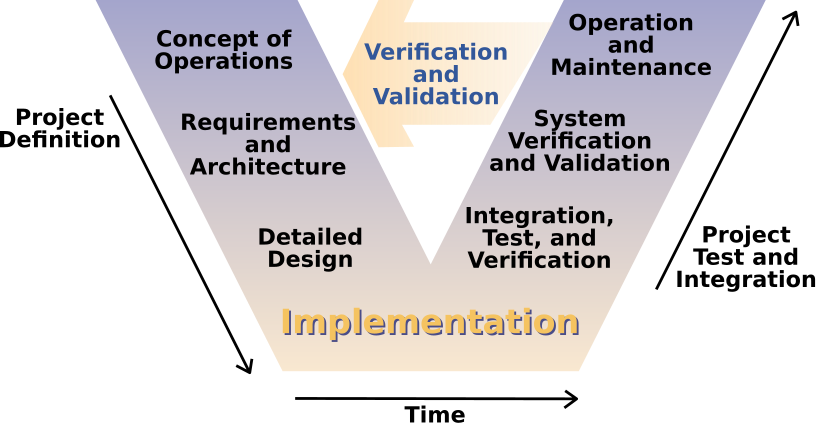
\includegraphics[width=\linewidth]{figures/v_model.png}
	\caption{V-Model}
	\label{fig:v_model}
\end{figure}

\parx
\textbf{Requirements.}
\justifying
Involves the gathering of data, analysis of the gathered data, and preparation
of the system requirements in defining the scope and features of the project.
This stage also involves the documentation of the requirements.

\parx
\textbf{System Design.}
\justifying
The documents created in the previous stage will be used to generate more
specific and technical documents and designs about the software to be developed
for this stage. The documents outline the components, modules, and high-level
guidelines for business logic.

\parx
\textbf{Architecture Design.}
\justifying
The technical designs from the System Design stage will be used to generate
specifications with lower level of technical details about the software and its
modules. The technology stack is also selected in this stage. During this stage,
the tests are also prepared for future use.

\parx
\textbf{Module Design.}
\justifying
In this stage, low-level designs are developed from the high-level designs
generated from previous stages. This will include specifications regarding each
individual module, component, interface, and so on. Unit tests are also prepared
in this stage.

\parx
\textbf{Implementation and Coding.}
\justifying
This stage the implementation through programming starts. It starts with coding
the each module individually with unit tests along applied following the designs
made in the initial stages of the development life cycle. Integration of the
modules to the system is done afterward and is run through system tests.

\parx
\textbf{Testings.}
\justifying
Tests are further applied to the system such as unit testing, integration
testing, system testing, and acceptance testing. Passing all these tests will be
considered as the verification and validation of the project.

	% \addcontentsline{toc}{subsection}{Context Diagram}
\flushleft
\textbf{Context Diagram}\\
\justifying

\parx
Context diagram is a simple diagram that shows the source systems contributing data to
a system as well as the major user constituents and downstream information systems
that it supports. This diagram is so simple that it makes it perfect for agile
requirement management. This diagram also called “Level 0” data flows diagrams because
if one were to put arrows on the connections between sources and targets, the diagram
could serve as the cover sheet of a data flow diagram packet that many analysts prepare
for traditionally managed projects. This diagram greatly reduce project risk because
they are easy for a team’s business partners to understand (\cite{hughes_2016}).

	% \addcontentsline{toc}{subsection}{Data Flow Diagram}
\flushleft
\textbf{Data Flow Diagram}\\
\justifying

\parx
A data flow diagram illustrates the processes, data stores, and external entities in
a business or other system and the connecting data flows. It is a graphical
representation of the flow of data through information system. DFD was first
proposed by Larry Constantine, the original developer of structured design in 1970s. It
is a primary artifact and is required to be created for every system in a structured
approach. It provides a different abstraction level that is useful in system designing
because of its hierarchical structure.  It shows data flow from external into the system
and shows how the data moved from one process to another. There are four symbols for
a data flow diagram: 1.) Squares or Ovals which represent external entities. It can be
a person or a group of people outside the control of the system being modeled. It shows
where information comes from and where it goes. 2.) Circles or Rounded Rectangles shapes
represent processes within the system. They show a part of the system that transforms
inputs to outputs. The name of the process  in the symbols usually explains what the
process does so that it is generally used with the verb-object phase. 3.) Arrows represents
how the data flows. It can be electronic data or physical items or both. The name of
the arrows represents the meaning of the packet that flows along. It also shows direction
to indicate whether data or items are moving out or into a process. The last symbol is
4.) Open-Ended Rectangles which represents data stores, including both electronic stores
and physical stores. Data stores might be used for accumulating data for a long or short
period of times (\cite{arwa_2016}).

	% \addcontentsline{toc}{subsection}{Gantt Chart}
\flushleft
\textbf{Gantt Chart}\\
\justifying

\parx
Gantt chart is a classic tool in project management. It is one of the most known and
widely used planning and management tool in projects in different domains. The
principles for the development and design of Gantt chart are time-focused, objective,
deterministic, analytic, accountable, and sequential
(\cite{geraldi_lechter_2012}).

\parx
Time-focus as projects have a target time for the either the completion or progress
milestone. Each task should be well coordinated in time and work as a crucial part in
project management.

\parx
Objective as projects must have ground in reality for the objectives to be met in a
realistic and feasible manner.

\parx
Deterministic as each task should be properly defined, studied, and defined. This
ensures that there should be no uncertainty in the objective and method of the tasks.

\parx
Analytical as projects are the sum of different and subset of tasks. A project must
be analyzed very well and divided properly into smaller tasks. This should take into
consideration the execution and scope of each task.

\parx
Accountable as a project gets divided into smaller parts, a project is also divided
and assigned to different person. Each person should be accountable for the progress
and completion of the task assigned.

\parx
Sequential as in the management of a project, there is always a sequence or order
required for further tasks to be started by waiting for the completion of other tasks
it depend upon. This sequence fit as a timeline analogy.

	% \addcontentsline{toc}{subsection}{Ishikawa Diagram}
\flushleft
\textbf{Ishikawa Diagram}\\
\justifying

\parx
Ishikawa diagram is also called the fishbone diagram and cause-and-effect diagram in
that it is a graphical technique in the shape of a fish skeleton used to numerous causes
of a phenomenon. It is commonly used to identify and analyze causes and its complex
relation to each other that contribute to the specific problem.

A finding of a study about the use of Ishikawa diagram as an appropriate theoretical
framework for representing visually and analyzing technology of complex factors of
major improvements and innovations over the course of history and time. This graphical
representation tool presents a simple and clear the order and relation of the causes
and roots of a problem addressed by the change in technology
(\cite{coccia_2017}).


	% \fakesubsection{Six Learning Barriers in End-User Programming Systems}
\flushleft
\textbf{Six Learning Barriers in End-User Programming Systems}\\
\justifying

\parx
The researchers identified the following aspects prone to false assumptions that include
fundamental and basic concepts in programming as barriers to learning programming.
These barriers closely related to the concept of interfaces of a programming environment
such as the constructs of the language itself and the availability of libraries,
features, and syntax that can be used to achieve desired procedures
(\cite{ko_myers_aung_2004}).

\parx
Design barriers are internal difficulties of a problem in programming. Solutions
to problems which are difficult to visualize affect the learning experience and may
lead to false assumptions and confusions.

\parx
Selection barriers occur when learners know what to do but are unable to identify which
of the available tools and features in the programming interface is to correct.

\parx
Coordination barriers are difficulties in using libraries provided by the programming
environment in compliment with another. Learner may know how to solve individual and
simple tasks but fails to combine the approaches to solve complex problems.

\parx
Use barriers are inherent to users new to the environment. The unfamiliarity to the
interface hinders its usage due to the lack of information and guide.

\parx
Understanding barriers involve the obscurity of the processes the programming interface
do that are hidden to the users. This occurs when learners fail to evaluate and
undestand the behavior of the program relative to their expectations.

\parx
Information barriers are difficulties in obtaining information about the internal
workings of the interface. This occurs when the environment provides no method for the
users to test their hypothesis regarding the behaviors of the environment.

\parx
The barriers explicitly defined are closely related to each other. The effect of having
difficulties in overcoming a barrier affects the learning of another barrier.

	% \fakesubsection{Visual Programming vs. Text-based Programming}
\flushleft
\textbf{Visual Programming vs. Text-based Programming}\\
\justifying

\parx
Programming is seen to be as the career of the future as technology continues to scale
up and improve. For this reason many countries are already promoting and implementing
programming subjects to their curriculum in primary education
(\cite{williams_alafghani_daley_gregory_rydzewski_2015}). Most of these formal subjects
use a visual programming language for teaching instead of the traditional text-based
programming language.

\parx
It would seem to be appropriate and more productive to teach
text-based language as it is the standard and the type of programming language used for
the development of softwares and applications in the industry and the real world.
However, in considering the comparison of the engagement, interest, and actual learning
of the students at the introductory level, visual programming language is more suited
and ideal as results showed that the motivation of the subjects that use visual
programming language improved (\cite{tsukamoto_2016}).

\parx
Studies also show that using a visual programming language like Scratch to teach
students programming and transitioning to real programming language (text-based) shows
a marginal improvements to their understanding of computer science concepts
(\cite{armoni_2015}). Visual-based environment as compared to textual
environment also displays positive results in terms of the interest and motivation of
the learners to pursue programming (\cite{daisuke_2017}).

\parx
Novice programmers take longer time to learn programming because of many constraints
that are needed to be learnt first such as the syntax and semantics of a programming
language. Common errors and difficulties in text-based programming languages include
type corrections, misspellings, typographical errors, and grammatical or syntax errors.
Another factor is that students whose native language is not English find it harder
to type because the keywords in most programming languages are in English. Even the
tools used, text editors or integrated development editors (IDE) are hard to operate
and use (\cite{liu_wu_dong_2010}).


	% \addcontentsline{toc}{subsection}{Prototype of Visual Programming Environment
% for C Language Novice Programmer}
\flushleft
\textbf{Prototype of Visual Programming Environment for C Language Novice
Programmer}\\
\justifying

\parx
The C programming language is often the first programming language taught and
learned in higher education. This is also the case for the author's institution,
the Kanagawa Institute of Technology - Department of Information Engineering.
The C language classes are thrice a week in the first year. The students use
Visual Studio for programming. In text-based languages like C, students must
memorize tokens or keywords such as data type and syntax in general. These are
difficulties for beginners. Even a single typographical error in text-based
programming can lead to undesirable messages like compilation errors.

\parx
The research and development of a programming support system for beginner
programmers has attained an advanced stage. One of which is the block-based
visual programming language environment such as Scratch or Snap!. Block-based
programming environments allow student to edit the program by visually selecting
blocks and combining them together. They can create programs even without the
need to memorize keywords or to understand the syntax in formulating the grammar
for the semantics. Scratch and Snap! use their own programming languages which
are not suitable for learning other popular languages like C, C++, or Java.

\parx
With these factors considered, in this investigation the researchers have
developed a visual programming environment for the C language with the goal of
lowering the barriers between starting in programming and learning of the C
programming language. This programming environment is a Web application that has
functions to edit a C language program and to execute and step through the
program and trace the changes in the variables (\cite{abe_fukawa_tanaka_2019}).

	% \fakesubsection{On the Design of a Generic Visual Programming Environment}
\flushleft
\textbf{On the Design of a Generic Visual Programming Environment}\\
\justifying

\parx
Visual programming languages are commonly embedded and coupled within
environments that are visually interactive. The identification of visual
programming language is associated with its environment. Therefore, the creation
of a visual programming language is tightly integrated with the creation of its
environment. The Requirements of a visual programming environment include
graphical elements with relationships graphically shown as each element is
connected with another element. Making an algorithm must be done graphically as
well through editing elements and creating connections between related data.
Each element contains underlying data structures that can be complex as there
are more information stored and used such as the visual representation, logical
connection, domain knowledge, and more. Parsing group of elements, or diagrams,
are difficult in that a parsing algorithm must be employed for handling such
case.

\parx
A generic visual programming environment can be represented as a group of
textual and visual specification tools. Designing a visual programming
environment requires consideration for the semantics and syntax of the language
as well as the visual interface. To handle with ease the maintenance,
modification, and reuse of a visual programming environment, modules are needed
to be specified clearly and with their interactions with one another
(\cite{da_qian_zhang_kang_zhang}).

	% \fakesubsection{Environment pi J for Visual Programming in Java}
\flushleft
\textbf{Environment pi J for Visual Programming in Java}\\
\justifying

\parx
There is a wide known visual tools for programming in Java such as Symantec
Cafe, Visual J++ by Microsoft, and Visual Age for Java by IBM. The main feature
of the tools listed is the possibility to modify the graphical elements of the
user interface. The tools support representation in graphic forms of program
structure for packages, classes, methods, and properties. The tools apply the
visual representation to view, modify, and debug the programs. There is a
difficulty to consider that is related to using the tools listed, and that is it
is necessary for the users to have relatively high knowledge in programming,
particularly in the Java programming language.

\parx
Pi J is a programming environment for developing professional software basing on
the concepts of object-oriented programming. Pi J can operate with two kinds of
file format and it allows opening and saving of text file in plain Java. It also
allows opening and saving of file as structured format that the tool can read.
The tool supports most of the features provided by the Java programming
language (\cite{prokhorov_kosarev}).

	% \fakesubsection{HASKEU: An editor to support visual and textual programming in tandem}
\flushleft
\textbf{HASKEU: An editor to support visual and textual programming in tandem}\\
\justifying

\parx
This paper shows the effectiveness and usefulness of combining textual and
visual system where a change between both system updates both interfaces. The
application of textual and visual systems in combination with one another allows
users and learners of programming to easily develop programs. Focusing on the
visual representation but at the same time seeing the textual representation.
This enables them to understand the effect of a change in both formats. Learning
through this will make it easier for learners to transition into more advance
and complex concepts. HASKEU was developed in a research project to assist
end-user functional programming for Haskell programs (\cite{alam_bush_2016}).

\parx
Learning programming is most times a time-consuming and frustrating task.
Writing and testing programs after the skills are learned can also be a
laborious endeavor. A textual program is one where the program presents a set
of commands in textual form for function and variable definition. Textual
programming tests our analytical, logical, and verbal thinking abilities. Visual
programming tests our non-verbal thinking ability as it uses meaningful
graphical representations. Visual representations assist learning and retention
in memory and may provide an incentive to learn programming without language
barriers.

\parx
In 1990, a committee of functional programmers created a well-developed and
powerful functional programming language called Haskell. Functional languages
are based on the lambda calculus. These mean that the programs have no concept
of state. Functional programs are pure functions which take input and produce an
output. In recent years, there is an increase in the usage of functional
programming but one thing to be considered is that functional programming can be
overwhelming to learn as it is very different to other more common type of
language such as declarative or imperative programming.

\parx
HASKEU is a prototype programming and development environment for the Haskell
programming language. This programming system was developed to support both
textual and visual programming. The HCI (HumanComputer Interaction) techniques
are used extensively by the design of HASKEU. The HCI techniques include rules
of design for UI, data display, icon, and direct manipulation.

	% \fakesubsection{The Scratch Programming Language and Environment}
\flushleft
\textbf{The Scratch Programming Language and Environment}\\
\justifying

\parx
The Scratch is visual programming language and environment that allows users to
create media-rich projects such as games and interactive media. Scratch is an
application that is used to create projects provided with media and scripts.
Assets like images and audio can be imported or created directly within the
application through the built-in paint and audio recorder tools. Any of these
things, that a text-based programming environment can, is possible through the
use of colorful command blocks to control graphical objects called sprites set
in a background called the stage
(\cite{maloney_resnick_rusk_silverman_eastmond_2010}).

\parx
Users learn Scratch as they use it, experimenting commands from the provided
palette or exploring projects from existing projects. Scratch was designed to
allow scripting, provide immediate feedback for the execution of scripts, and
making the execution and data visible to motivate users for such self-directed
learning. The following are the design followed by Scratch:

\parx
\textbf{Single-Window user interface.}
The user interface of Scratch makes
navigation easier as it only uses a single window with multiple panes to ensure
that key components are always visible.

\parx
\textbf{Liveness and Tinkerability.}
One of the key features of Scratch is that it is always live. There is no
compilation phase. The program listens to each interaction between the user and
the interface and process it accordingly to provide smoother experience and
immediate feedback to the users.

\parx
\textbf{Making Execution Visible.}
Scratch provides feedback visually to show the execution of scripts. There is an
indicator around the script element for users to easily identify and follow it.
This feature helps users understand the flow of the program such as when it is
triggered and the duration of the script.

\parx
\textbf{No Error Messages.}
When people play with blocks such as LEGO, there is no error message
encountered. Blocks fit together only in certain ways, and it is easier to get
things right than wrong. The shapes of the block suggest the possible position
and orientation for it to properly fit and experimentation and experience teach
what works and what does not.

\parx
\textbf{Making Data Concrete}.
In most programming languages, variables are abstract and harder to understand.
Scratch turns variables into concrete objects that the user sees and
manipulates, through tinkering and observation making programming easier to
understand.

\parx
\textbf{Minimizing the Command Set}.
Scratch aims to minimize the number of command blocks while still allowing a
wide range of project types. One might point out that flexibility, convenience
of the programmers, and more features are better than a small set of commands.
In Scratch, every command consumes screen space in the command palettes, so
there is more cost to increasing the set of commands. Addition of more commands
requires additional categories or forcing the user to navigate and scroll down
to see all the commands available within a given group.

	% \fakesubsection{CodeMonkey}
\flushleft
\textbf{CodeMonkey}\\
\justifying

\parx
CodeMonkey is a learning environment for developing computational thinking aimed
primarily at elementary and secondary school students. This learning environment
follows the context of game-based and challenge-based learning methodology.
CodeMonkey is different than common block-based programming approach like Scratch
in that students are required to input code at the initial phase of the game.
Nevertheless, no prior programming knowledge is required. Learners need to aid
a monkey, the main character, in catching bananas while facing various challenges
and obstacles. There are multiple worlds, each with theme and set of challenges,
progressing from one world to another is only possible if the learner completes
the previous world and its challenges. Users may submit a solution to a challenge,
then the system automatically checks it and responds with immediate feedback based
on the submission. Feedback includes stars which act as rewards to further
motivate the learner into solving more challenges (\cite{codemonkey_2020}).


\end{doublespace}


	\clearpage
	\begin{doublespace}
	\begin{center}
		\section*{METHODOLOGY}
	\end{center}

	\leavevmode\\
	\par
	\justifying
	This chapter shows the materials and methods that the researchers will use
	for the development of CodeNect: Visual Programming Software for Learning
	Fundamentals of Programming.

	\flushleft
\textbf{Materials}\\
\justifying

\parx
For the development of CodeNect: Visual Programming Software for Learning
Fundamentals of Programming, the researchers use the following specifications:

\parx
For the software requirements, the following materials are used in the
development of the software: Linux 5.4 Kernel with Manjaro distrubution as
Operating System, Terminal for running commands, Vim for text and code editor,
Kha for the graphical, media, and control framework, zui for the base
user-interface, and C++ as programming language. The following are used for the
deployment of the software: Microsoft Windows 7 and above, C++ Runtime
libraries, and the C++ programming language.

\parx
For the hardware requirements, the following materials are used in the
development of the software: Laptop with 2 GB of RAM (Random Access Memory),
processor of Intel Core 2 Duo (1.4 GHz), and storage of 80 GB HDD (Hard Disk
Drive). The following materials are used for the deployment of the software: at
least Intel Core 2 Duo at 1.4 GHz, 2 GB of RAM, and 1 GB HDD of storage.

	\flushleft
\textbf{Method}\\
\justifying

\parx
The researchers will use the V-Model methodology of Software
Development Life Cycle (SDLC) for the proposed software to be developed. The
V-Model methodology is a linear development methodology that focuses and follows
a strict and incremental steps of stages. The initial phases are generally
focused on planning and designing the system, the next phases are focused on
implementation and actual programming. After that, the model will go in upwards
direction for testing and verification of the project. The development of the
software follows the timeline (See Appendix Figure \ref{fig:gantt_chart}).

\parx
The V-Model figure shows the following stages:

\flushleft
\textbf{Requirements.}
\justifying
\parx
In this stage the researchers conducted a survey to gather data from
students, instructors, and learners in the field of technology and under the
course with programming subjects such as Bachelor of Science in Information
Technology, Bachelor of Science in Computer Science, and Bachelor of Science in
Computer Engineering as respondents. The data gathered
(See Appendix Figure \ref{dataresults1})
are evaluated and assessed to determine the knowledge and understanding of
the respondents in regards to the fundamentals of programming, experience and
feedback on traditional text-based tools and software. Problems are identified
and the Ishikawa Diagrams are constructed
(See Appendix Figure \ref{fishbone1}, \ref{fishbone2}, and
\ref{fishbone3}).

\flushleft
\textbf{System Design.}
\justifying
The researchers will assess the gathered data and study the information in order
to construct a context diagram representing the manual way that the study will
solve (See Appendix Figure \ref{fig:context_diagram_manual}). The schedule of the
development and the allotted time for each is task is planned through the Gantt
chart (See Appendix Figure \ref{fig:gantt_chart}).

\flushleft
\textbf{Architecture Design.}
\justifying
\parx
The researchers in this stage will design and develop specifications that will
serve as the blueprint of the software. The libraries, packages, tools, and more
are will be finalized and prepared for later use
(See Appendix Figure \ref{fig:context_diagram}).

\flushleft
\textbf{Module Design.}
\justifying
\parx
The researchers will identify and define the scopes and specific features of
each module and how will each be integrated along the system to work with other
modules and components to ensure that each module is decoupled and can be tested
without dependency in other module
(See Appendix Figure \ref{fig:theoretical_framework}).

\flushleft
\textbf{Implementation and Coding.}
\justifying
\parx
The researchers will start to program each module in the C++ programming
language using Vim as the primary text editor. Compiling and running the
software will be done by running a command in the terminal. The rendering
backend will be OpenGL and the GLFW for the windowing and input framework. Each
functionality of each module will be tested using unit tests by running the
test every functionality that will be implemented.  After each module passes
the associated test, all will be coupled and integrated to a single system. The
end product of this phase is the CodeNext: Visual Programming Software for
Learning Fundamentals of Programming.

\flushleft
\textbf{Testing.}
\justifying
\parx
The researchers will apply tests in the software that will be developed.
Further testings will be done. Bugs, errors, and misbehaviors will be handled
and fixed. This test will ensure that the functionality, efficiency,
usability, portability, and reliability of the software meets the standard.

\flushleft
\textbf{Evaluation.}
\justifying
\parx
The evaluation to be used is the ISO/IEC/IEEE 29119-4:2015. The respondents
will test the software thoroughly to specifically evaluate their experience and
their learning.
The respondents will be asked to use both traditional text-based programming and the
CodeNect: Visual Programming Software in a period of a week each. After that, the
respondents will be tasked to solve simple coding exercises. After that, the
respondents will be given a feedback form to assess their experience with both
tools and the researchers will evaluate their solutions to the coding exercises
and compare the results.


\end{doublespace}


	\clearpage
	\begin{doublespace}
		\fakesection{\textbf{REFERENCES}}
		\printbibliography[title={\center{REFERENCES}}]
	\end{doublespace}

  \clearpage
	\begin{center}
		\section{\textbf{APPENDIX FIGURES}}
	\end{center}
  \begin{doublespace}
	\begin{center}
		\app{Survey and Assessment Form}

		% \subsection*{APPENDIX A} \label{appendixa}
		\null\vfill\appendixform{1}{1}\vfill
		\null\vfill\appendixform{1}{2}\vfill
		\null\vfill\appendixform{1}{3}\vfill
		\null\vfill\appendixform{1}{5}\vfill
		\null\vfill\appendixform{1}{5}\vfill
		\null\vfill\appendixform{1}{6}\vfill
		\null\vfill\appendixform{1}{7}\vfill
		\null\vfill\appendixform{1}{8}\vfill
		\null\vfill\appendixform{1}{9}\vfill
		\null\vfill\appendixform{1}{11}\vfill
		\appfig{Assessment Form}
		\null\vfill\appendixform{2}{1}\vfill
		\null\vfill\appendixform{2}{2}\vfill
		\null\vfill\appendixform{2}{3}\vfill
		\null\vfill\appendixform{2}{4}\vfill
		\null\vfill\appendixform{2}{5}\vfill
		\appfig{Survey Form}

		\app{Graphical Representation of Data}
		\renewcommand{\figurename}{Appendix Figure}

		\clearpage
		\null\vfill
		\appendixdata{1}
		\appfig{Graphical representation of the course of the respondents}
		\label{dataresults1}
		\vfill
		\appendixdata{2}
		\appfig{Graphical representation of the grade/year level of the respondents}
		\label{dataresults2}
		\vfill

		\clearpage
		\null\vfill
		\appendixdata{3}
		\appfig{Graphical representation of the desired field in technology to work in of the respondents}
		\label{dataresults3}
		\vfill
		\appendixdata{4}
		\appfig{Graphical representation of the knowledge of programming before college of the respondents}
		\label{dataresults4}
		\vfill

		\clearpage
		\null\vfill
		\appendixdata{5}
		\appfig{Graphical representation of the years programming of the respondents}
		\label{dataresults5}
		\vfill
		\appendixdata{6}
		\appfig{Graphical representation of the languages comfortable with of the respondents}
		\label{dataresults6}
		\vfill

		\clearpage
		\null\vfill
		\appendixdata{7}
		\appfig{Graphical representation of the education method for learning best of the respondents}
		\label{dataresults7}
		\vfill
		\appendixdata{8}
		\appfig{Graphical representation of the hard to learn in programming of the respondents}
		\label{dataresults8}
		\vfill

		\clearpage
		\null\vfill
		\appendixdata{9}
		\appfig{Graphical representation of the text-editing tool used of the respondents}
		\label{dataresults9}
		\vfill
		\appendixdata{10}
		\appfig{Graphical representation of the alternative method preferred in learning of the respondents}
		\label{dataresults10}
		\vfill

		\clearpage
		\null\vfill
		\appendixdata{11}
		\appfig{Graphical representationa of the ease of usage and favor with text-based editors of the respondents}
		\label{dataresults11}
		\vfill
		\appendixdata{12}
		\appfig{Graphical representation of the understanding of programming fundamentals of the respondents}
		\label{dataresults12}
		\vfill

		\clearpage
		\null\vfill
		\appendixdata{13}
		\appfig{Graphical representation of the assessment of programming fundamentals knowledge of the respondents}
		\label{dataresults13}
		\vfill

		% \subsection*{APPENDIX C} \label{ishikawadiagrams}
		% \subsubsection*{Ishikawa Diagrams}
		\clearpage
		\null\vfill
		\app{Ishikawa Diagram}
		\begin{figure}[H]
			\centering
			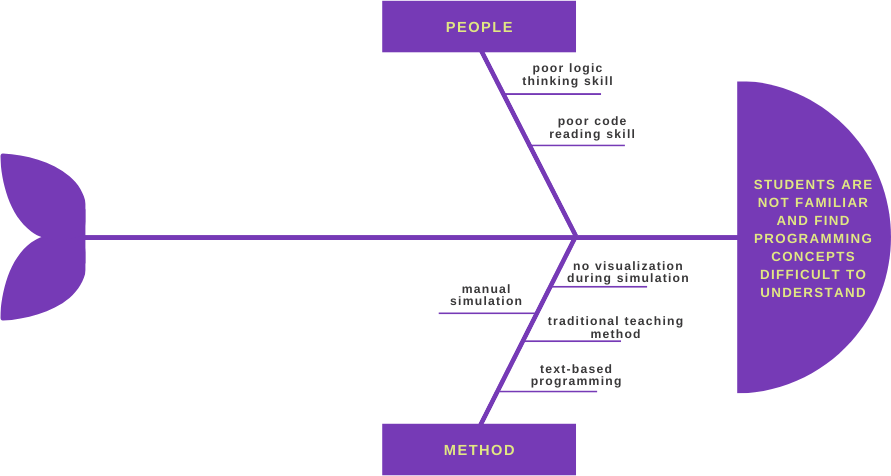
\includegraphics[width=0.8\textheight,angle=90]{figures/fishbone1.png}
			% \caption[Ishikawa Diagram 1]{Fishbone diagram of the students are not familiar and find
			% programming concepts difficult to understand}
			\label{fig:fishbone1}
		\end{figure}
		\appfig{Fishbone diagram of the students are not familiar and find programming concepts difficult to understand}
		\vfill

		\clearpage
		\null\vfill
		\begin{figure}[H]
			\centering
			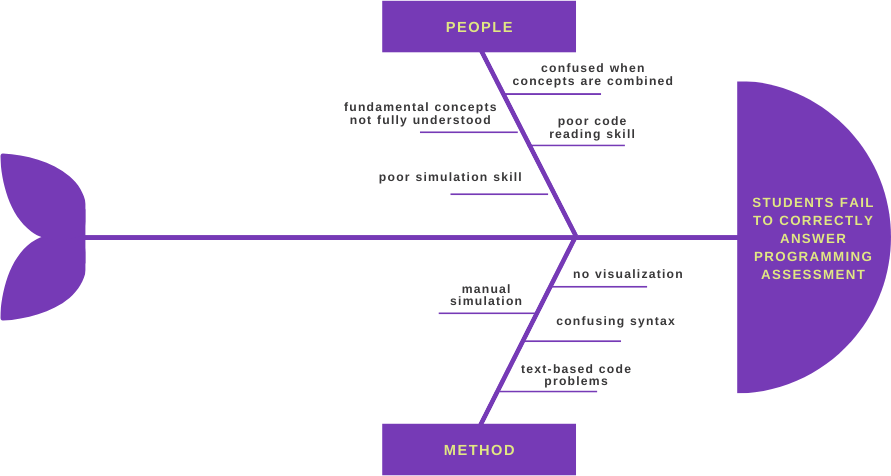
\includegraphics[width=0.8\textheight,angle=90]{figures/fishbone2.png}
			% \caption[Ishikawa Diagram 2]{Fishbone diagram of the students fail to correctly answer programming
			% assessment}
			\label{fig:fishbone2}
		\end{figure}
		\appfig{Fishbone diagram of the students fail to correctly answer programming assessment}
		\vfill

		\clearpage
		\null\vfill
		\begin{figure}[H]
			\centering
			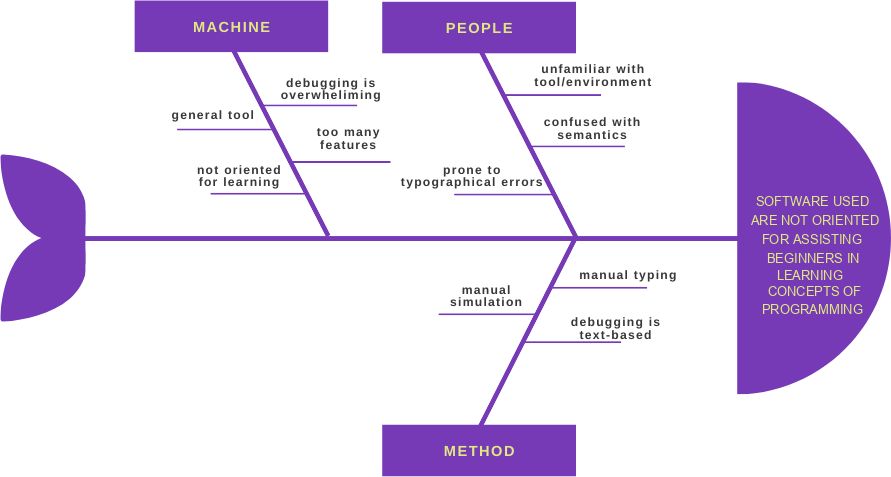
\includegraphics[width=0.8\textheight,angle=90]{figures/fishbone3.png}
			% \caption[Ishikawa Diagram 3]{Fishbone diagram of the tool for programming not effective for
			% learning}
			\label{fig:fishbone3}
		\end{figure}
		\appfig{Fishbone diagram of the tool for programming not effective for learning}
		\vfill

		% \appendix
		% \subsection*{APPENDIX D} \label{appendixc}
		% \subsubsection*{Context Diagram (Manual)} \label{contextdiagrammanual}
		\clearpage
		\null\vfill
		\app{Context Diagram}
		\begin{figure}[H]
			\centering
			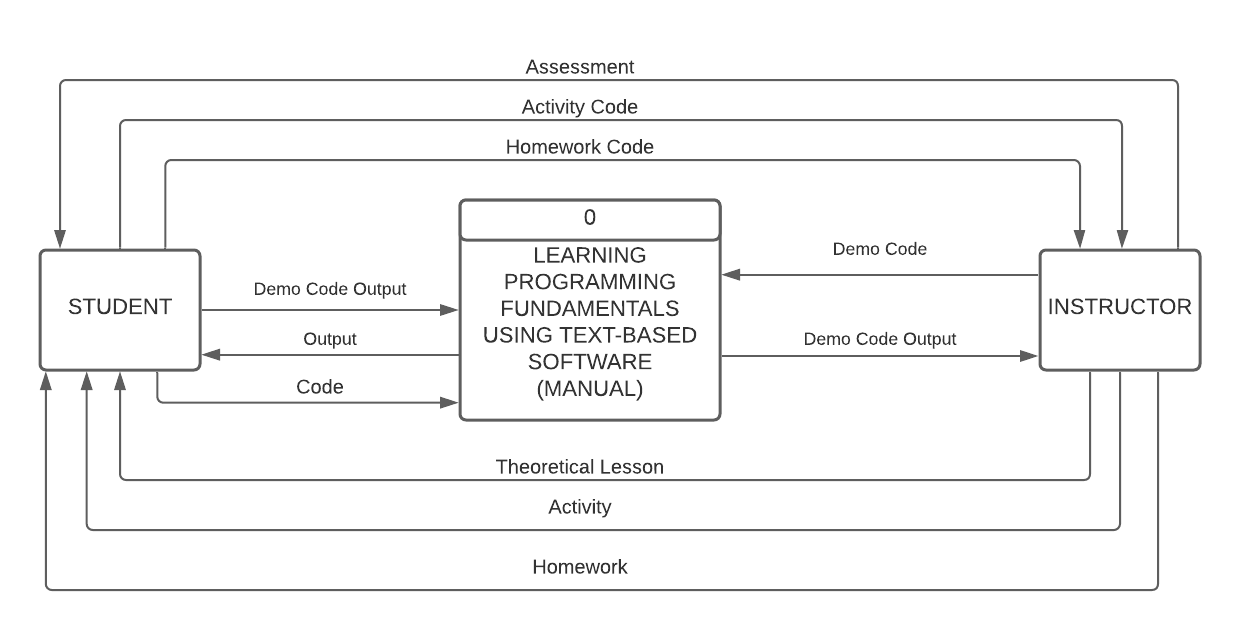
\includegraphics[width=\textwidth]{figures/context_diagram_manual.png}
			% \caption{Context Diagram of Existing System}
			\label{fig:context_diagram_manual}
		\end{figure}
		\appfig{Context Diagram of Existing System}
		\vfill

		% \subsubsection*{Context Diagram} \label{contextdiagram}
		\begin{figure}[H]
			\centering
			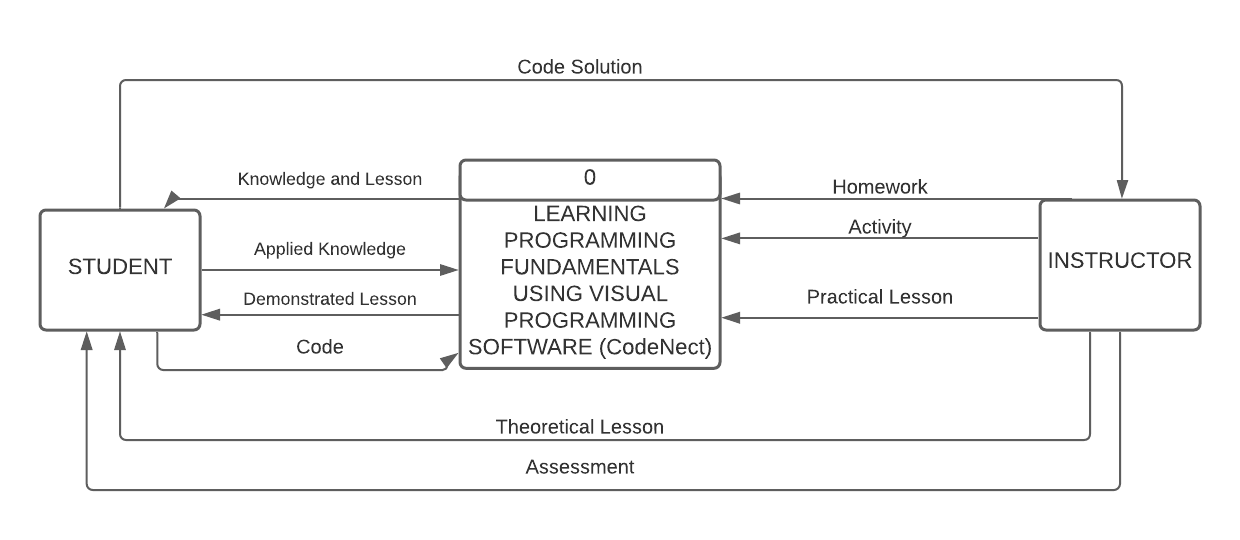
\includegraphics[width=\textwidth]{figures/context_diagram.png}
			% \caption{Context Diagram of Proposed System}
			\label{fig:context_diagram}
		\end{figure}
		\appfig{Context Diagram of Proposed System}
		\vfill

		% \subsection*{APPENDIX E} \label{ganttchart}
		% \subsubsection*{Gantt Chart}
		% \begin{figure}[H]
		% 	\centering
		% 	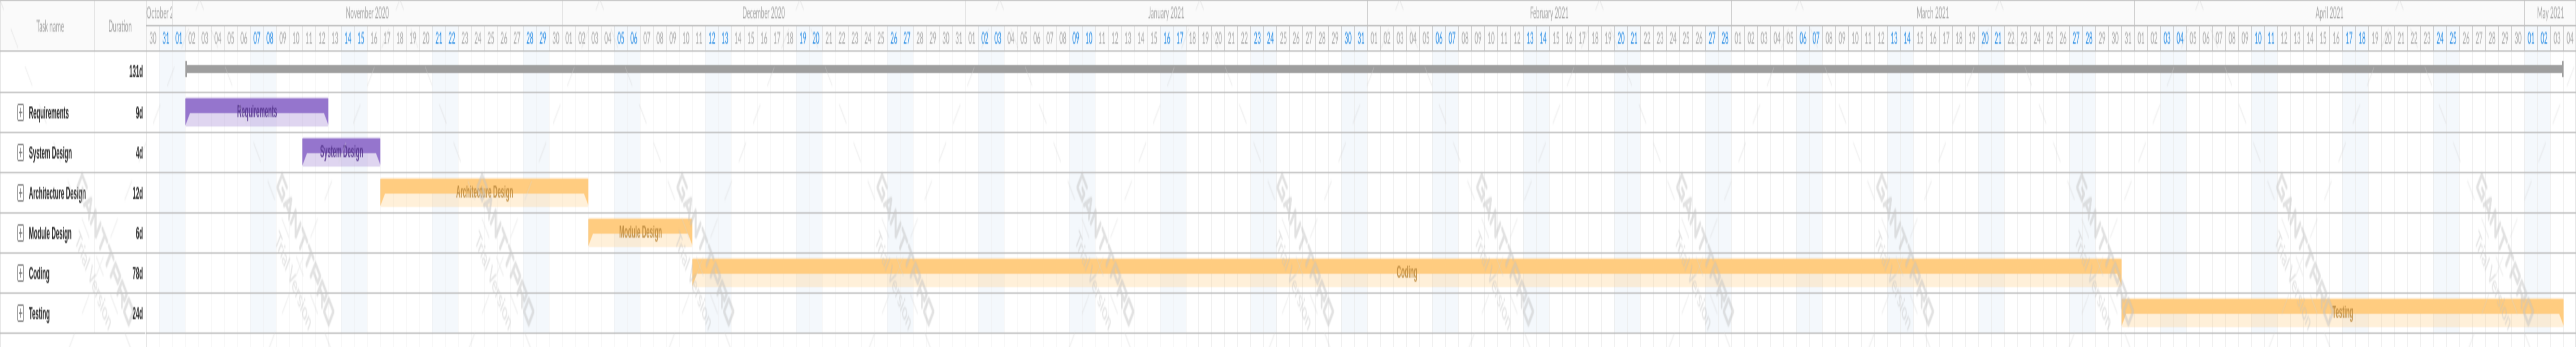
\includegraphics[width=0.8\textheight,angle=90]{figures/gantt_chart.png}
		% 	\caption[Gantt Chart]{Gantt Chart of the Development of CodeNect}
		% 	\label{fig:gantt_chart}
		% \end{figure}

		\app{Gantt Chart}
		\begin{sidewaysfigure}
			\centering
			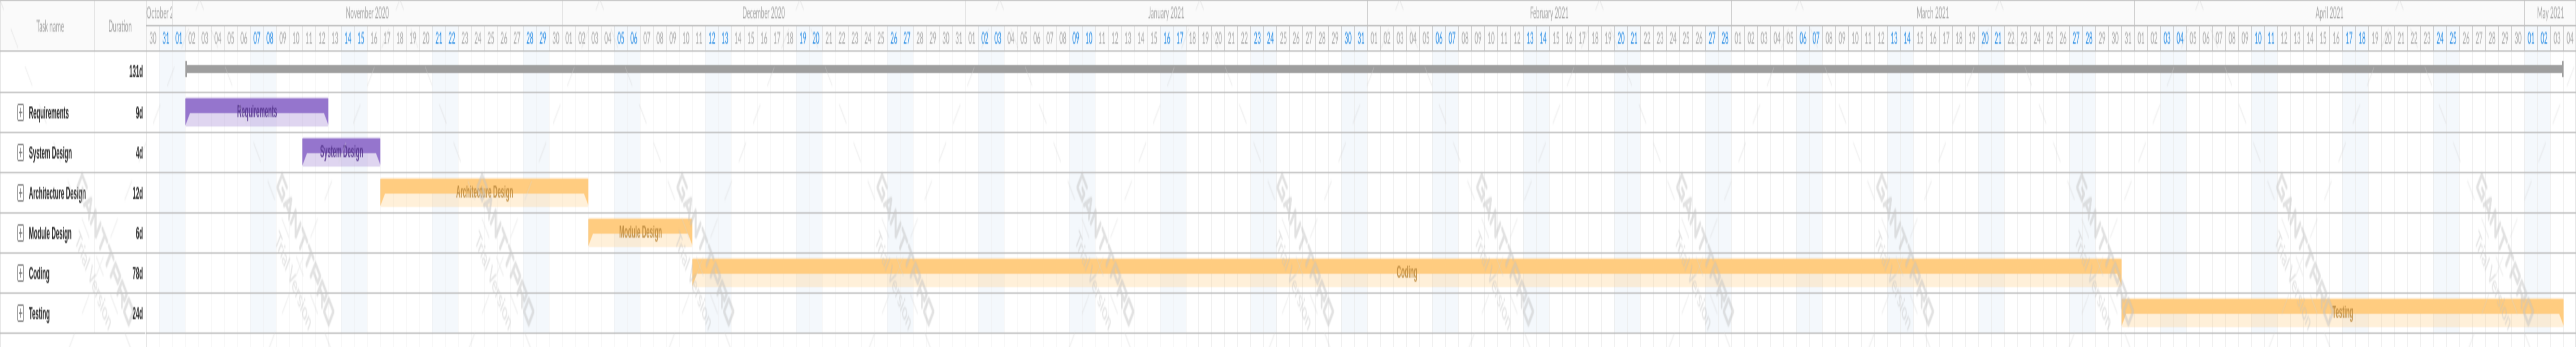
\includegraphics[width=0.8\textwidth]{figures/gantt_chart.png}
			% \caption[Gantt Chart]{Gantt Chart of the Development of CodeNect}
			\label{fig:gantt_chart}
			\appfig{Gantt Chart of the Development of CodeNect}
		\end{sidewaysfigure}
		\vfill

		\clearpage
		\null\vfill
		% \subsection*{APPENDIX F} \label{theoreticalframework}
		% \subsubsection*{Theoretical Framework}
		\app{Theoretical Framework}
		\begin{figure}[H]
			\centering
			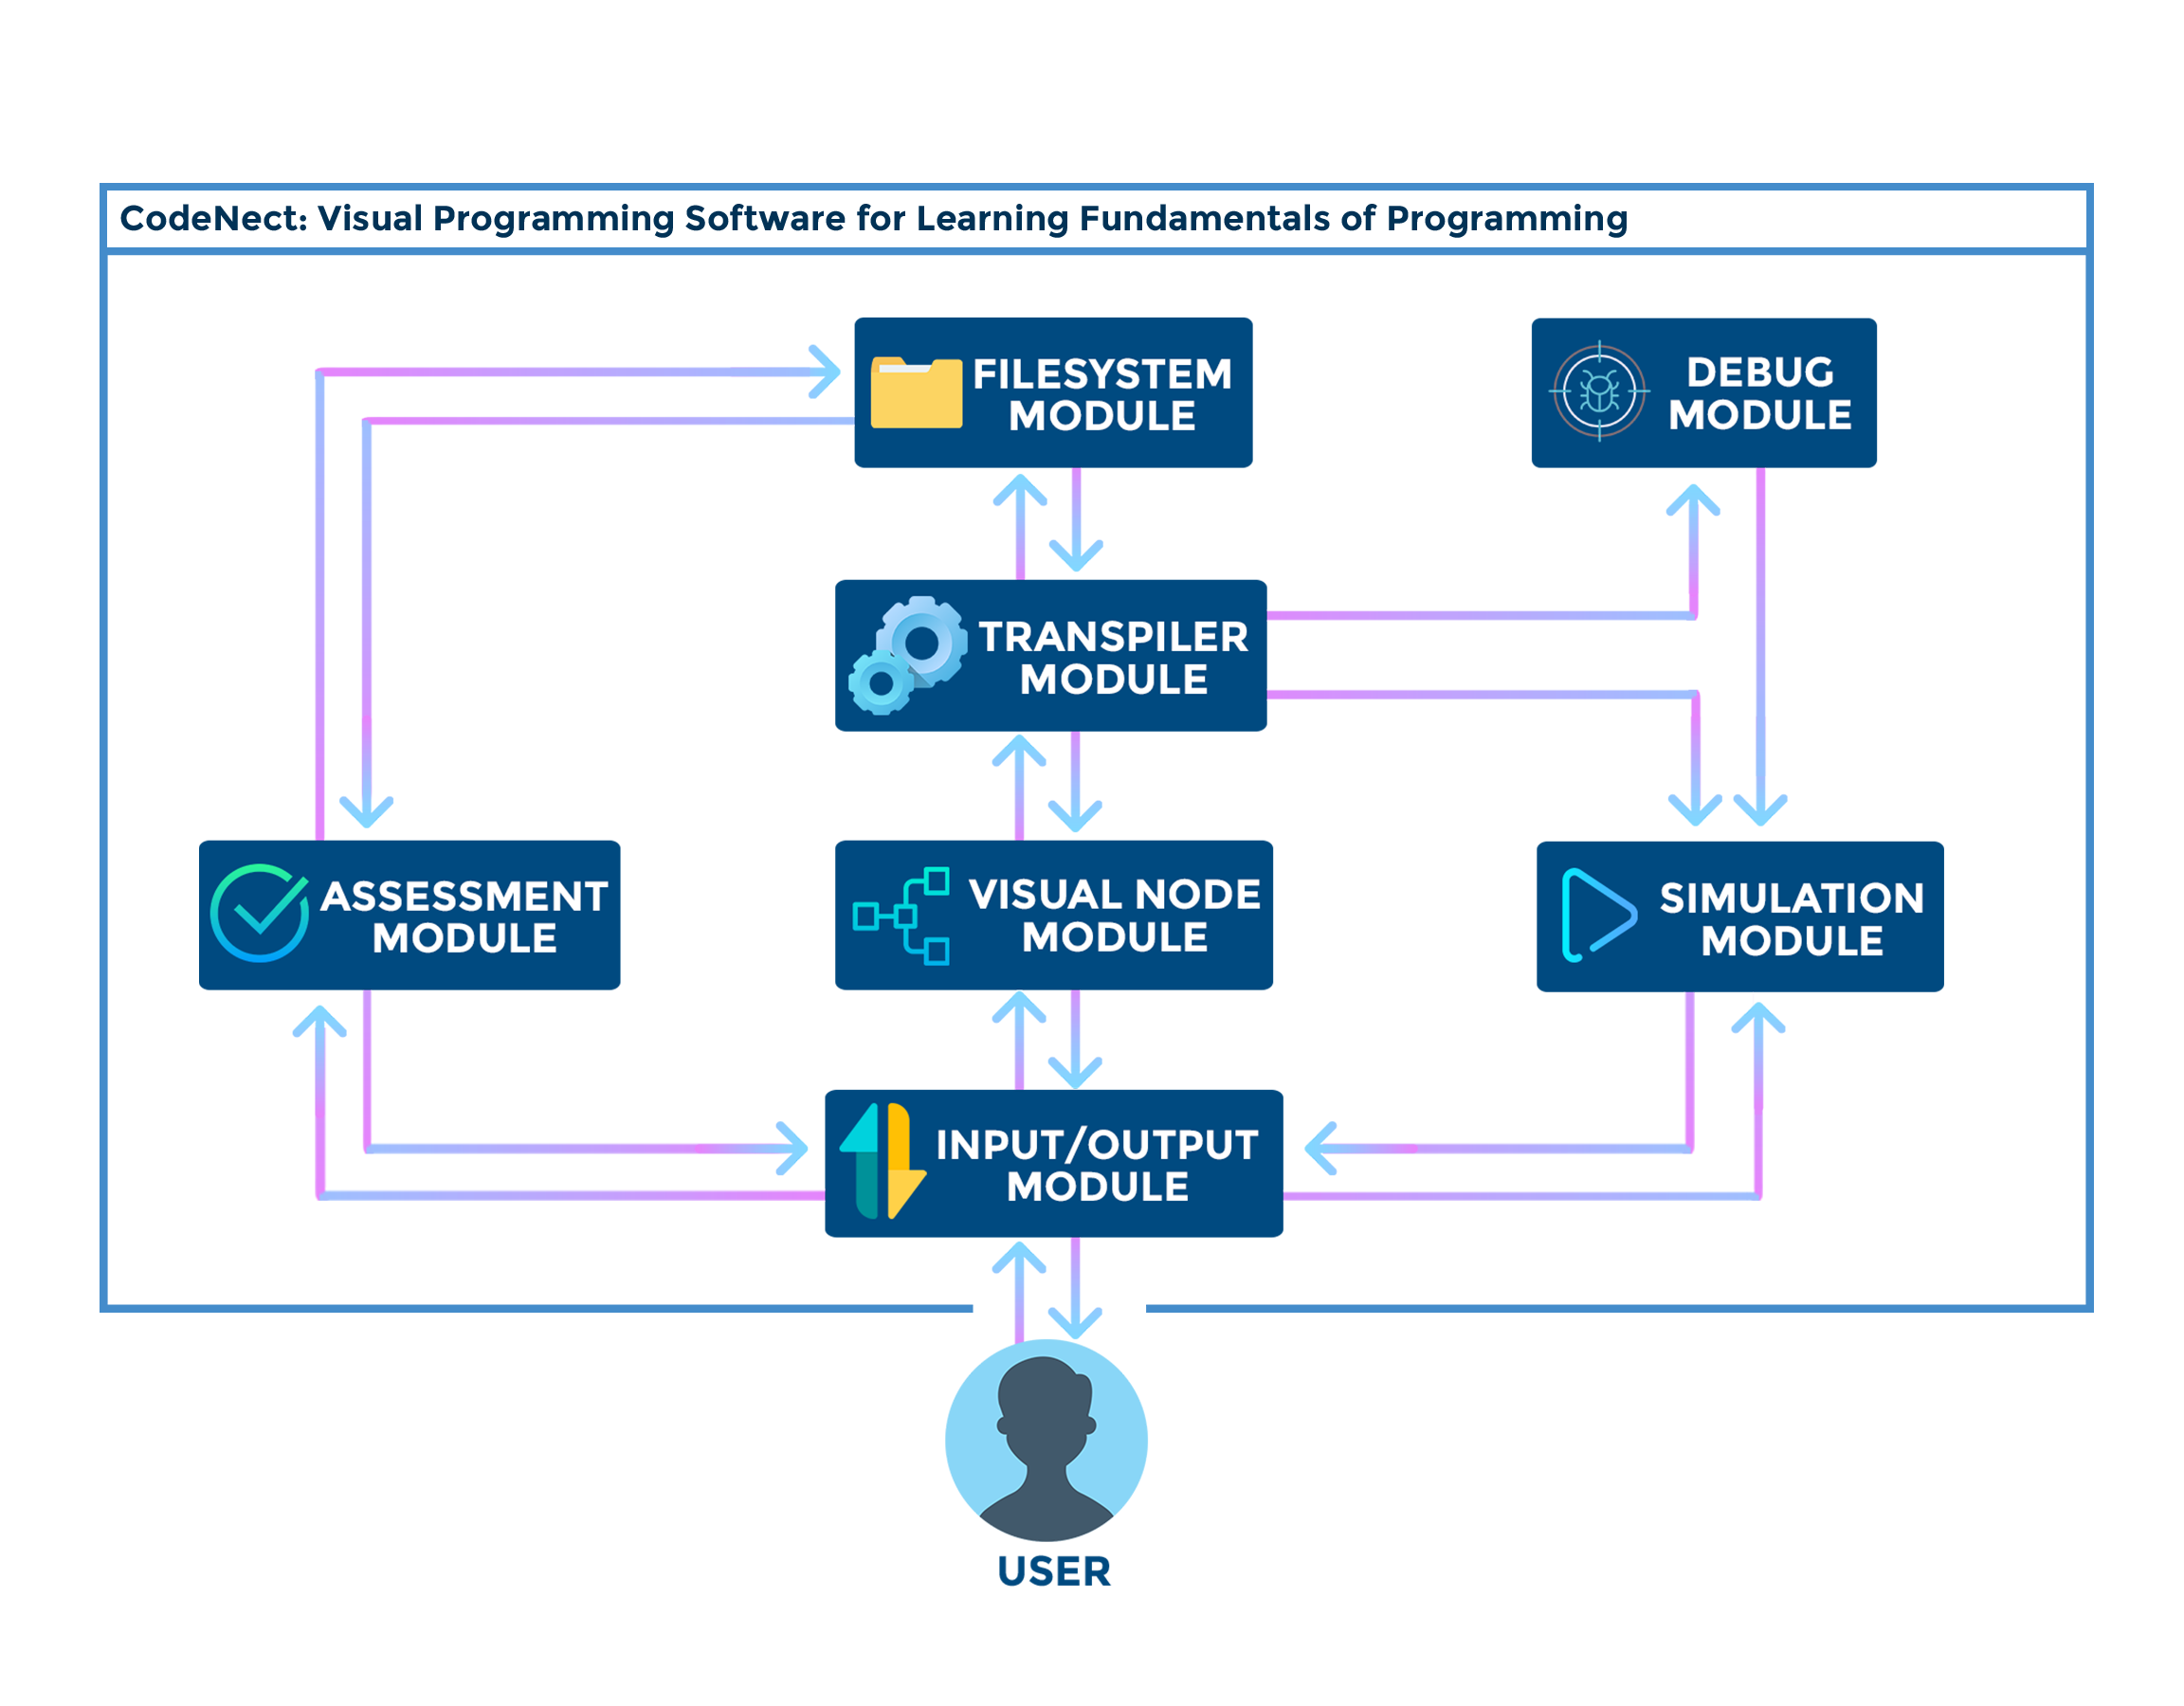
\includegraphics[width=\textwidth]{figures/theoretical_framework.png}
			% \caption[Theoretical Framework]{Theoretical Framework of CodeNect: Visual Programming Software
			% for Learning Fundamentals of Programming}
			\label{fig:theoretical_framework}
		\end{figure}
		\appfig{Theoretical Framework of CodeNect: Visual Programming Software for Learning Fundamentals of Programming}
		\vfill

	\end{center}
\end{doublespace}

\end{document}
